%%%%%%%%%%%%%%%%%%%%%%%%%%%%%%%%%%%%%%%%%%%%%%%%%%%%%%%%%%%%%%%%%%%%%%%%%%%%%%%
%% Plantilla de memoria en LaTeX para la ETSIT - Universidad Rey Juan Carlos
%%
%% Por Gregorio Robles <grex arroba gsyc.urjc.es>
%%     Grupo de Sistemas y Comunicaciones
%%     Escuela Técnica Superior de Ingenieros de Telecomunicación
%%     Universidad Rey Juan Carlos
%% (muchas ideas tomadas de Internet, colegas del GSyC, antiguos alumnos...
%%  etc. Muchas gracias a todos)
%%
%% La última versión de esta plantilla está siempre disponible en:
%%     https://github.com/gregoriorobles/plantilla-memoria
%%
%% Para obtener PDF, ejecuta en la shell:
%%   make
%% (las imágenes deben ir en PNG o JPG)

%%%%%%%%%%%%%%%%%%%%%%%%%%%%%%%%%%%%%%%%%%%%%%%%%%%%%%%%%%%%%%%%%%%%%%%%%%%%%%%%

\ifdefined\printedVersion
  \documentclass[a4paper, 12pt]{book}
\else
  \documentclass[a4paper, 12pt, oneside, openany]{book}
\fi
%\usepackage[T1]{fontenc}
%\usepackage[utf8]{inputenc}


%\usepackage[T1]{fontenc} 
%\usepackage[utf8]{inputenc}
%\PrerenderUnicode{ÁáÉéÍíÓóÚúÑñ} % Para que salgan las tildes y demás mierdas en el título.

\usepackage{exmath}


\RequirePackage{MathUnicode} % Paquete para poder poner caracteres griegos y demás cosas raras.


%\ifdefined\printedVersion
%  \usepackage[a4paper, left=3.8cm, right=2.5cm, top=3.3cm, bottom=3cm,headsep=1cm,headheight=3cm]{geometry}
%\else
\usepackage[a4paper, left=3cm, right=3cm, top=3.3cm, bottom=3cm,headsep=1cm,headheight=3cm]{geometry}
%\fi

\usepackage{times}

%\usepackage[utf8]{inputenc}
\usepackage[spanish,es-tabla]{babel} % Comenta esta línea si tu memoria es en inglés
\usepackage{url}
%\usepackage[dvipdfm]{graphicx}
\usepackage{graphicx}
\usepackage{float}  %% H para posicionar figuras
\usepackage[nottoc, notlot, notlof, notindex]{tocbibind} %% Opciones de índice
\usepackage{latexsym}  %% Logo LaTeX

\usepackage{amsmath} % Matemáticas
\usepackage{amsfonts} % Mas Matemáticas
\usepackage{amssymb} % Mas Matemáticas
\usepackage{amsthm} % Otro paquete de Matemáticas
\usepackage[shadow]{todonotes} % Marcas To Do (a hacer)
\usepackage{xspace} % Espaciado correcto detras de comandos.
\usepackage{mathtools} % Arregla bastantes cosas de los entornos matemáticos por 
\usepackage[acronym]{glossaries} % Glosarios
\usepackage{makeidx}
\usepackage[breaklinks=true,
			pdfauthor={V\'ictor de Juan},
            pdftitle={Trabajo de Fin de M\'aster},
            pdfsubject={Gamificaci\'on},
            pdfkeywords={Gamificaci\'on, Educaci\'on, Matem\'aticas}]{hyperref}
			
\usepackage{breakcites} % Permite romper citas en saltos de línea.
\usepackage{enumitem}
\usepackage{multirow}
\usepackage{graphicx}

\usepackage{array}
\usepackage{placeins}
\usepackage{flafter}
\usepackage{fancyhdr}
\usepackage{newtxmath,newtxtext}
\usepackage{seqsplit}
\usepackage{titlesec} 
\usepackage{hyperref}

\usepackage{soulutf8}
%\renewcommand{\todo}[1]{\hl{(#1)}}

\usepackage{tocvsec2} % Ignorar subsecciones de los anexos.
\usepackage{appendix} % Cambiar apéndice por anexo.
\settocdepth{subsection} 


%\usepackage{longtable}
\usepackage{booktabs}
\usepackage{ltablex}



\usepackage{footnote}
\makesavenoteenv{tabular}
\makesavenoteenv{table}


\usepackage{pdfpages}

%%%%%%%%%%%%%%%%%%%%%%%%%%%%%%%%%%%%%%%%%%%%%%%%%%%%%%%%%%%%%%%%%%%%%%%%%%
%%%%%%%%%%%%%%%%%%%%%%%%%%%%%%%%%%%%%%%%%%%%%%%%%%%%%%%%%%%%%%%%%%%%%%%%%%
%%%%%%%%%%%%%%%%%%%%%%%%%%%%%%%%%%%%%%%%%%%%%%%%%%%%%%%%%%%%%%%%%%%%%%%%%%
%%%%%%%%%%%%%%%%%%%%%         TÍTULOS         %%%%%%%%%%%%%%%%%%%%%%%%%%%
%%%%%%%%%%%%%%%%%%%%%%%%%%%%%%%%%%%%%%%%%%%%%%%%%%%%%%%%%%%%%%%%%%%%%%%%%%
%%%%%%%%%%%%%%%%%%%%%%%%%%%%%%%%%%%%%%%%%%%%%%%%%%%%%%%%%%%%%%%%%%%%%%%%%%
%%%%%%%%%%%%%%%%%%%%%%%%%%%%%%%%%%%%%%%%%%%%%%%%%%%%%%%%%%%%%%%%%%%%%%%%%%
%%%%%%%%%%%%%%%%%%%%%%%%%%%%%%%%%%%%%%%%%%%%%%%%%%%%%%%%%%%%%%%%%%%%%%%%%%

 
\newcommand{\nombreautor}{V\'ictor de Juan Sanz\xspace}
\newcommand{\nombretutor}{Desir\'e Garc\'ia L\'azaro\xspace}
\newcommand{\titulo}{Gamificaci\'on: visión general y aplicación en el aula de Matemáticas\xspace}
\newcommand{\TFM}{Trabajo Fin de M\'aster\xspace}
\newcommand{\master}{M\'aster Universitario en Formaci\'on del Profesorado de Educación Secundaria Obligatoria y Bachillerato, Formación Profesional y Enseñanza de Idiomas\xspace}
\newcommand{\especialidad}{Matem\'aticas}
%\newcommand{\master}{Máster en Formación del Profesorado: especialidad Matemáticas}






%%%%%%%%%%%%%%%%%%%%%%%%%%%%%%%%%%%%%%%%%%%%%%%%%%%%%%%%%%%%%%%%%%%%%%%%%%
%%%%%%%%%%%%%%%%%%%%%%%%%%%%%%%%%%%%%%%%%%%%%%%%%%%%%%%%%%%%%%%%%%%%%%%%%%
%%%%%%%%%%%%%%%%%%%%%%%%%%%%%%%%%%%%%%%%%%%%%%%%%%%%%%%%%%%%%%%%%%%%%%%%%%
%%%%%%%%%%%%%%%%            Header y Footer           %%%%%%%%%%%%%%%%%%%%
%%%%%%%%%%%%%%%%%%%%%%%%%%%%%%%%%%%%%%%%%%%%%%%%%%%%%%%%%%%%%%%%%%%%%%%%%%
%%%%%%%%%%%%%%%%%%%%%%%%%%%%%%%%%%%%%%%%%%%%%%%%%%%%%%%%%%%%%%%%%%%%%%%%%%
%%%%%%%%%%%%%%%%%%%%%%%%%%%%%%%%%%%%%%%%%%%%%%%%%%%%%%%%%%%%%%%%%%%%%%%%%%
%%%%%%%%%%%%%%%%%%%%%%%%%%%%%%%%%%%%%%%%%%%%%%%%%%%%%%%%%%%%%%%%%%%%%%%%%%



%\pagestyle{fancy}
%\fancyhf{}

\renewcommand{\headrulewidth}{0.4pt}
\renewcommand{\headrule}{{
\vspace{0.3cm}\hrule width\headwidth height\headrulewidth \vskip-\headrulewidth}}

\renewcommand{\thesection}{\thechapter.\arabic{section}}




\titleformat{\chapter}
  {\normalfont\fontsize{12}{15}\bfseries}{\thechapter.}{0.5em}{}
\titlespacing*{\chapter}{0pt}{3.5ex plus 1ex minus .2ex}{2.3ex plus .2ex}

\titleformat{\section}
  {\normalfont\fontsize{12}{15}\bfseries}{\thesection}{1em}{}

\titleformat{\subsection}
  {\normalfont\fontsize{12}{15}\bfseries}{\thesubsection}{1em}{}

\titleformat{\subsubsection}
  {\normalfont\fontsize{12}{15}\bfseries}{\thesubsubsection}{1em}{}


\renewcommand{\cfttoctitlefont}{\normalfont\fontsize{12}{15}\bfseries}
\renewcommand{\cftaftertoctitle}{\hfill}
\setlength{\cftbeforetoctitleskip}{20pt}
\setlength{\cftaftertoctitleskip}{10pt}

\renewcommand\cftloftitlefont{\normalfont\fontsize{12}{15}\bfseries}
\renewcommand{\cftafterloftitle}{\hfill}
\setlength{\cftbeforeloftitleskip}{20pt}
\setlength{\cftafterloftitleskip}{10pt}

\renewcommand\cftlottitlefont{\normalfont\fontsize{12}{15}\bfseries}
\renewcommand{\cftafterlottitle}{\hfill}
\setlength{\cftbeforelottitleskip}{20pt}
\setlength{\cftafterlottitleskip}{10pt}


%\renewcommand{\cfttoftitlefont}{\normalfont\fontsize{12}{15}\bfseries}
%\renewcommand{\cfttoltitlefont}{\normalfont\fontsize{12}{15}\bfseries}




\newcommand{\righthead}{\raisebox{1.15\height}{\nombreautor\quad}}
\newcommand{\lefthead}{\raisebox{-0.13\height}{\quad
\includegraphics[height=15mm]{img/Logo_header.png}}}
\newcommand{\centerhead}{Gamificaci\'on: visión general y\\
aplicación en el aula de Matemáticas}

%\fancyhead[LE,RO]{\righthead}\fancyhead[RE,LO]{\lefthead}\fancyhead[CE,CO]{\centerhead}\fancyfoot[CE,CO]{\thepage}


\rhead{\righthead}
\lhead{\lefthead}
\chead{\centerhead}
\cfoot{\thepage}


\renewcommand{\baselinestretch}{1.5}  %% Interlineado

\setlist{topsep=0ex,itemsep=-1ex,partopsep=1ex,parsep=1ex}


%%%%%%%%%%%%%%%%%%%%%%%%%%%%%%%%%%%%%%%%%%%%%%%%%%%%%%%%%%%%%%%%%%%%%%%%%%
%%%%%%%%%%%%%%%%%%%%%%%%%%%%%%%%%%%%%%%%%%%%%%%%%%%%%%%%%%%%%%%%%%%%%%%%%%
%%%%%%%%%%%%%%%%%%%%%%%%%%%%%%%%%%%%%%%%%%%%%%%%%%%%%%%%%%%%%%%%%%%%%%%%%%
%%%%%%%%%%%%%%%%%            Bibliografía           %%%%%%%%%%%%%%%%%%%%%%
%%%%%%%%%%%%%%%%%%%%%%%%%%%%%%%%%%%%%%%%%%%%%%%%%%%%%%%%%%%%%%%%%%%%%%%%%%
%%%%%%%%%%%%%%%%%%%%%%%%%%%%%%%%%%%%%%%%%%%%%%%%%%%%%%%%%%%%%%%%%%%%%%%%%%
%%%%%%%%%%%%%%%%%%%%%%%%%%%%%%%%%%%%%%%%%%%%%%%%%%%%%%%%%%%%%%%%%%%%%%%%%%
%%%%%%%%%%%%%%%%%%%%%%%%%%%%%%%%%%%%%%%%%%%%%%%%%%%%%%%%%%%%%%%%%%%%%%%%%%


\newcommand{\ign}[1]{}

\addto\captionsspanish{
   \renewcommand{\BOthers}[1]{et al.\hbox{}}%
}
\usepackage{apacite}
\addto\captionsspanish{
   \renewcommand{\BOthers}[1]{et al.\hbox{}}%
}
\bibliographystyle{apacite}

\addto\captionsspanish{
   \renewcommand{\BOthers}[1]{et al.\hbox{}}%
}
\usepackage[sort&compress]{natbib}
\usepackage{usebib}


\addto\captionsspanish{
   \renewcommand{\BOthers}[1]{et al.\hbox{}}%
}


\interfootnotelinepenalty=10000



\newcommand{\citePisa}[1]{(\gls{PISA}, #1)}

%%%%%%%%%%%%%%%%%%%%%%%%%%%%%%%%%%%%%%%%%%%%%%%%%%%%%%%%%%%%%%%%%%%%%%%%%%
%%%%%%%%%%%%%%%%%%%%%%%%%%%%%%%%%%%%%%%%%%%%%%%%%%%%%%%%%%%%%%%%%%%%%%%%%%
%%%%%%%%%%%%%%%%%%%%%%%%%%%%%%%%%%%%%%%%%%%%%%%%%%%%%%%%%%%%%%%%%%%%%%%%%%
%%%%%%%%%%%%%%%%%            ABREVIATURAS           %%%%%%%%%%%%%%%%%%%%%%
%%%%%%%%%%%%%%%%%%%%%%%%%%%%%%%%%%%%%%%%%%%%%%%%%%%%%%%%%%%%%%%%%%%%%%%%%%
%%%%%%%%%%%%%%%%%%%%%%%%%%%%%%%%%%%%%%%%%%%%%%%%%%%%%%%%%%%%%%%%%%%%%%%%%%
%%%%%%%%%%%%%%%%%%%%%%%%%%%%%%%%%%%%%%%%%%%%%%%%%%%%%%%%%%%%%%%%%%%%%%%%%%
%%%%%%%%%%%%%%%%%%%%%%%%%%%%%%%%%%%%%%%%%%%%%%%%%%%%%%%%%%%%%%%%%%%%%%%%%%

\newcommand{\arab}{al-Karaji\xspace}
\newcommand{\Arab}{Al-Karaji\xspace}
\newcommand{\logro}[2]{\labeltext{#1\xspace}{logro::#2} #1\xspace}


\newif\ifincgls
\incglsfalse

\newif\ifboe
\boefalse
  
\newif\ifbocm
\bocmfalse
  
\newif\iflomce
\lomcefalse
  

\ifincgls

  
  \newcommand{\crossref}[1]{#1} % Incluimos referencias cruzadas.


  % Incluimos glosario.
  \newcommand{\boe}{\gls{BOE}}
  \newcommand{\lomce}{\gls{LOMCE}}
  \newcommand{\bocm}{\gls{BOCM}}
  \newcommand{\eaes}{\glspl{EAE}}
  \newcommand{\eae}{\gls{EAE}}

\else
  
  \newcommand{\crossref}[1]{} % Ignoramos referencias cruzadas.
  

  % Chapuza por no utilizar glosarios.
  \defcitealias{LOMCE}{Ley Org\'anica 8/2013, de 9 de diciembre, para la Mejora de la Calidad Educativa}
  \defcitealias{BOE}{Real Decreto 1105/2014, de 26 de diciembre, por el que se establece el curr\'iculo b\'asico de la Educaci\'on Secundaria Obligatoria y del Bachillerato}
  \defcitealias{BOCM}{Decreto 48/2015, de 14 de mayo, del Consejo de Gobierno, por el que se establece para la Comunidad de Madrid el curr\'iculo de la Educaci\'on Secundaria Obligatoria}


  \newcommand{\boe}{
    \ifboe
        BOE\xspace
    \else
      \citetalias{BOE} (de ahora en adelante BOE)\xspace
      \boetrue
    \fi}

  \newcommand{\bocm}{
    \ifbocm
        BOCM\xspace
    \else
      \citetalias{BOCM} (de ahora en adelante BOCM)\xspace
      \bocmtrue
    \fi}

  \newcommand{\lomce}{
    \iflomce
        LOMCE\xspace
    \else
      \citetalias{LOMCE} (de ahora en adelante LOMCE)\xspace
      \lomcetrue
    \fi}

  % Más chapuzas
  \newcommand{\eaes}{Estándares de Aprendizaje Evaluables\xspace}
  \newcommand{\eae}{Estándar de Aprendizaje Evaluable\xspace}

\fi




%%%%%%%%%%%%%%%%%%%%%%%%%%%%%%%%%%%%%%%%%%%%%%%%%%%%%%%%%%%%%%%%%%%%%%%%%%
%%%%%%%%%%%%%%%%%%%%%%%%%%%%%%%%%%%%%%%%%%%%%%%%%%%%%%%%%%%%%%%%%%%%%%%%%%
%%%%%%%%%%%%%%%%%%%%%%%%%%%%%%%%%%%%%%%%%%%%%%%%%%%%%%%%%%%%%%%%%%%%%%%%%%
%%%%%%%%%%%%%%%%%%             Renombrando           %%%%%%%%%%%%%%%%%%%%%
%%%%%%%%%%%%%%%%%%%%%%%%%%%%%%%%%%%%%%%%%%%%%%%%%%%%%%%%%%%%%%%%%%%%%%%%%%
%%%%%%%%%%%%%%%%%%%%%%%%%%%%%%%%%%%%%%%%%%%%%%%%%%%%%%%%%%%%%%%%%%%%%%%%%%
%%%%%%%%%%%%%%%%%%%%%%%%%%%%%%%%%%%%%%%%%%%%%%%%%%%%%%%%%%%%%%%%%%%%%%%%%%
%%%%%%%%%%%%%%%%%%%%%%%%%%%%%%%%%%%%%%%%%%%%%%%%%%%%%%%%%%%%%%%%%%%%%%%%%%



\renewcommand{\cftfigfont}{Figura }
\renewcommand{\cfttabfont}{Tabla }
\renewcommand{\appendixname}{Anexos}
\renewcommand{\appendixtocname}{Anexos}
\renewcommand{\appendixpagename}{Anexos}


% Keywords (español e inglés)
\def\keywordsEn{\vspace{5em}
{\textbf{\textit{Key words ---}}\,\relax%
}}
\def\endkeywordsEn{\par}

\def\keywordsEs{\vspace{5em}
{\textbf{\textit{Palabras clave ---}}\,\relax%
}}
\def\endkeywordsEs{\par}



%%%%%%%%%%%%%%%%%%%%%%%%%%%%%%%%%%%%%%%%%%%%%%%%%%%%%%%%%%%%%%%%%%%%%%%%%%
%%%%%%%%%%%%%%%%%%%%%%%%%%%%%%%%%%%%%%%%%%%%%%%%%%%%%%%%%%%%%%%%%%%%%%%%%%
%%%%%%%%%%%%%%%%%%%%%%%%%%%%%%%%%%%%%%%%%%%%%%%%%%%%%%%%%%%%%%%%%%%%%%%%%%
%%%%%%%%%%%%%%%%%%%%%%%         SAGE         %%%%%%%%%%%%%%%%%%%%%%%%%%%%%
%%%%%%%%%%%%%%%%%%%%%%%%%%%%%%%%%%%%%%%%%%%%%%%%%%%%%%%%%%%%%%%%%%%%%%%%%%
%%%%%%%%%%%%%%%%%%%%%%%%%%%%%%%%%%%%%%%%%%%%%%%%%%%%%%%%%%%%%%%%%%%%%%%%%%
%%%%%%%%%%%%%%%%%%%%%%%%%%%%%%%%%%%%%%%%%%%%%%%%%%%%%%%%%%%%%%%%%%%%%%%%%%
%%%%%%%%%%%%%%%%%%%%%%%%%%%%%%%%%%%%%%%%%%%%%%%%%%%%%%%%%%%%%%%%%%%%%%%%%%

 
\DeclareFixedFont{\ttb}{T1}{txtt}{bx}{n}{9} % for bold
\DeclareFixedFont{\ttm}{T1}{txtt}{m}{n}{9}  % for normal
% Defining colors
\usepackage{color}
\definecolor{deepblue}{rgb}{0,0,0.5}
\definecolor{deepred}{rgb}{0.6,0,0}
\definecolor{deepgreen}{rgb}{0,0.5,0}


\usepackage{listings}

% Python style for highlighting
\newcommand\pythonstyle{\lstset{
  language=Python,
  backgroundcolor=\color{white}, %%%%%%%
  basicstyle=\ttm,
  otherkeywords={self},            
  keywordstyle=\ttb\color{deepblue},
  emph={MyClass,__init__},          
  emphstyle=\ttb\color{deepred},    
  stringstyle=\color{deepgreen},
  commentstyle=\color{red},  %%%%%%%%
  frame=tb,                         
  lineskip={-1.5pt},
  breaklines=true,
  postbreak=\raisebox{0ex}[0ex][0ex]{\ensuremath{\color{red}\hookrightarrow\space}},
  showstringspaces=false
}}

% Python environment
\lstnewenvironment{python}[1][]
{
\pythonstyle
\lstset{#1}
}
{}




%%%%%%%%%%%%%%%%%%%%%%%%%%%%%%%%%%%%%%%%%%%%%%%%%%%%%%%%%%%%%%%%%%%%%%%%%%
%%%%%%%%%%%%%%%%%%%%%%%%%%%%%%%%%%%%%%%%%%%%%%%%%%%%%%%%%%%%%%%%%%%%%%%%%%
%%%%%%%%%%%%%%%%%%%%%%%%%%%%%%%%%%%%%%%%%%%%%%%%%%%%%%%%%%%%%%%%%%%%%%%%%%
%%%%%%%%%%%%%%%%%%%%             OTROS           %%%%%%%%%%%%%%%%%%%%%%%%%
%%%%%%%%%%%%%%%%%%%%%%%%%%%%%%%%%%%%%%%%%%%%%%%%%%%%%%%%%%%%%%%%%%%%%%%%%%
%%%%%%%%%%%%%%%%%%%%%%%%%%%%%%%%%%%%%%%%%%%%%%%%%%%%%%%%%%%%%%%%%%%%%%%%%%
%%%%%%%%%%%%%%%%%%%%%%%%%%%%%%%%%%%%%%%%%%%%%%%%%%%%%%%%%%%%%%%%%%%%%%%%%%
%%%%%%%%%%%%%%%%%%%%%%%%%%%%%%%%%%%%%%%%%%%%%%%%%%%%%%%%%%%%%%%%%%%%%%%%%%

\newcommand{\comillas}[1]{“#1”}
\newcommand{\Justificacion}[1]{\textit{Fundamentación teórica\xspace#1:}\xspace}


\renewcommand{\concept}[2][None]{
  \text{#2}% IGN
  %\marginpar{\footnotesize \textit{\makefirstuc{#2}}}%
  \renewcommand{\IS}{!}%
  \ifthenelse{\equal{#1}{None}}{\index{#2}}{\index{#1}}}


\newcommand{\coment}[1]{\textit{#1}}
\renewcommand{\coment}[1]{}


\newcommand{\mylabel}[2]{#2\def\@currentlabel{#2}\labeltext{#2}{#1}}
\MakeRobust{\ref}% avoid expanding it when in a textual label
\makeatletter
\newcommand{\labeltext}[2]{%
  \@bsphack
  \csname phantomsection\endcsname % in case hyperref is used
  \def\@currentlabel{#1}{\label{#2}}%
  \@esphack
}
\makeatother

\titleformat{\paragraph}[hang]{\normalfont\normalsize\bfseries}{\theparagraph}{-0.6em}{}
%\titlespacing*{\paragraph}{0pt}{3.25ex plus 1ex minus .2ex}{0.5em}

\newif\ifinapp
\inapptrue


%%%%%%%%%%%%%%%%%%%%%%%%%%%%%%%%%%%%%%%%%%%%%%%%%%%%%%%%%%%%%%%%%%%%%%%%%%
%%%%%%%%%%%%%%%%%%%%%%%%%%%%%%%%%%%%%%%%%%%%%%%%%%%%%%%%%%%%%%%%%%%%%%%%%%
%%%%%%%%%%%%%%%%%%%%%%%%%%%%%%%%%%%%%%%%%%%%%%%%%%%%%%%%%%%%%%%%%%%%%%%%%%
%%%%%%%%%%%%%%%%%%%%             Kahoot            %%%%%%%%%%%%%%%%%%%%%%%
%%%%%%%%%%%%%%%%%%%%%%%%%%%%%%%%%%%%%%%%%%%%%%%%%%%%%%%%%%%%%%%%%%%%%%%%%%
%%%%%%%%%%%%%%%%%%%%%%%%%%%%%%%%%%%%%%%%%%%%%%%%%%%%%%%%%%%%%%%%%%%%%%%%%%
%%%%%%%%%%%%%%%%%%%%%%%%%%%%%%%%%%%%%%%%%%%%%%%%%%%%%%%%%%%%%%%%%%%%%%%%%%
%%%%%%%%%%%%%%%%%%%%%%%%%%%%%%%%%%%%%%%%%%%%%%%%%%%%%%%%%%%%%%%%%%%%%%%%%%

\usepackage{tikz}
\newcommand*\circled[1]{\tikz[baseline=(char.base)]{
            \node[shape=circle,draw,inner sep=2pt] (char) {#1};}}

\newcommand{\correcta}[1]{\circled{#1}}
\newcounter{bloq}[section]
\renewcommand{\thebloq}{\arabic{section}.\alph{bloq}}
\newcounter{preg}[bloq]
\newcommand{\newbloq}{\setcounter{preg}{1}\stepcounter{bloq}\paragraph{Bloque \thebloq:}\xspace}
\renewcommand{\thepreg}{\alph{bloq}.\arabic{preg}}
\newcommand{\newpreg}[2]{
  \stepcounter{preg}
  \textbf{Pregunta \thepreg} \textit{(por valor de #1 puntos)}:
  #2
  }


%%%%%%%%%%%%%%%%%%%%%%%%%%%%%%%%%%%%%%%%%%%%%%%%%%%%%%%%%%%%%%%%%%%%%%%%%%
%%%%%%%%%%%%%%%%%%%%%%%%%%%%%%%%%%%%%%%%%%%%%%%%%%%%%%%%%%%%%%%%%%%%%%%%%%
%%%%%%%%%%%%%%%%%%%%%%%%%%%%%%%%%%%%%%%%%%%%%%%%%%%%%%%%%%%%%%%%%%%%%%%%%%
%%%%%%%%%%%%%%%%%%             Glosarios           %%%%%%%%%%%%%%%%%%%%%%%
%%%%%%%%%%%%%%%%%%%%%%%%%%%%%%%%%%%%%%%%%%%%%%%%%%%%%%%%%%%%%%%%%%%%%%%%%%
%%%%%%%%%%%%%%%%%%%%%%%%%%%%%%%%%%%%%%%%%%%%%%%%%%%%%%%%%%%%%%%%%%%%%%%%%%
%%%%%%%%%%%%%%%%%%%%%%%%%%%%%%%%%%%%%%%%%%%%%%%%%%%%%%%%%%%%%%%%%%%%%%%%%%
%%%%%%%%%%%%%%%%%%%%%%%%%%%%%%%%%%%%%%%%%%%%%%%%%%%%%%%%%%%%%%%%%%%%%%%%%%


\makeglossaries
\newacronym{FPGA}{FPGA}{Field-Programmable Gate Array}

% Glosario

% TODO: Añadir aqu\'i las definiciones del glosario
% Ejemplo de glosario
\newglossaryentry{bitstream}{name={bitstream},description={En este contexto se refiere al binario que configura el Hardware de la FPGA}}



\newacronym{PISA}{PISA}{\textit{Programme for International Student Assessment}}
\newacronym{TIMSS}{TIMSS}{\textit{Trends in International Mathematics and Science Study}}

\newacronym{INEE}{INEE}{Instituto Nacional de Evaluaci\'on Educativa}
\newacronym{INTEF}{INTEF}{Instituto Nacional de Tecnolog\'ias Educativas y Formaci\'on del Profesorado}


\newacronym{PDA}{PDA}{Programaci\'on Did\'actica Anual}


\newacronym{PBL}{PBL}{\textit{Points, Badges and Leaderboards} (Puntos, Medallas y Rankings)}

\newacronym{MUD}{MUD}{\textit{MultiUser Dungeon} -- juegos de rol online}

\newacronym{WCW}{WCW}{\textit{World Gamification Congress} -- Barcelona}

\newglossaryentry{real number}
{
  name={real number},
  description={include both rational numbers, such as $42$ and 
               $\frac{-23}{129}$, and irrational numbers, 
               such as $\pi$ and the square root of two; or,
               a real number can be given by an infinite decimal
               representation, such as $2.4871773339\ldots$ where
               the digits continue in some way; or, the real
               numbers may be thought of as points on an infinitely
               long number line},
  symbol={\ensuremath{\mathbb{R}}}
}

\newacronym{MOOC}{MOOC}{\textit{Massive Online Open Course} -- Curso masivo abierto en l\'inea}

\newacronym{TIC}{TIC}{Tecnolog\'ias de la Informaci\'on y de la Comunicaci\'on}

\makeindex

\newif\iftocs
\tocstrue % Incluye en el índice general: la lista de tablas, lista de figuras y acrónimos.
\tocsfalse % Excluye en el índice general: la lista de tablas, lista de figuras y acrónimos.



\begin{document}
\renewcommand{\BOthers}[1]{et al.\hbox{}}
\renewcommand{\BAvailFrom}[1]{Recuperado de\hbox{}}
\renewcommand{\BRetrievedFrom}[1]{Recuperado de }
\renewcommand{\BRetrieved}[1]{}
\renewcommand{\bibname}{Bibliografía}


%%%%%%%%%%%%%%%%%%%%%%%%%%%%%%%%%%%%%%%%%%%%%%%%%%%%%%%%%%%%%%%%%%%%%%%%%%%%%%%%
%%%%%%%%%%%%%%%%%%%%%%%%%%%%%%%%%%%%%%%%%%%%%%%%%%%%%%%%%%%%%%%%%%%%%%%%%%%%%%%%
% PORTADAS Y DEMÁS %
%%%%%%%%%%%%%%%%%%%%%%%%%%%%%%%%%%%%%%%%%%%%%%%%%%%%%%%%%%%%%%%%%%%%%%%%%%%%%%%%


\pagenumbering{Roman} % para empezar la numeración de página con números
\renewcommand{\refname}{Bibliografía}  %% Renombrando
\renewcommand{\appendixname}{Apéndice}

%%%%%%%%%%%%%%%%%%%%%%%%%%%%%%%%%%%%%%%%%%%%%%%%%%%%%%%%%%%%%%%%%%%%%%%%%%%%%%%%
% PORTADA

\begin{titlepage}
\begin{center}
\begin{tabular}[c]{c c}
%\includegraphics[bb=0 0 194 352, scale=0.25]{logo} &
\includegraphics[scale=0.25]{img/logo_vect.png} &
\begin{tabular}[b]{l}
\Huge
\textsf{UNIVERSIDAD} \\
\Huge
\textsf{REY JUAN CARLOS} \\
\end{tabular}
\\
\end{tabular}

\vspace{3cm}

\master

\vspace{0.4cm}

\large
Curso Académico 2016/2017

\vspace{0.8cm}

\TFM

\vspace{2.5cm}

\LARGE
\textsc{\titulo}

\vspace{4cm}

\large
Autor : \nombreautor \\
Tutor : \nombretutor
\end{center}
\end{titlepage}

\newpage
\mbox{}
\thispagestyle{empty} % para que no se numere esta pagina


%%%%%%%%%%%%%%%%%%%%%%%%%%%%%%%%%%%%%%%%%%%%%%%%%%%%%%%%%%%%%%%%%%%%%%%%%%%%%%%%
%%%% Para firmar
\clearpage
%\pagenumbering{gobble}
\chapter*{}
\thispagestyle{empty} % para que no se numere esta pagina

\vspace{-4cm}
\begin{center}
\LARGE
\textbf{\TFM}

\vspace{1cm}
\large
\titulo

\vspace{1cm}
\large
\textbf{Autor :} \nombreautor \\
\textbf{Tutor :} \nombretutor

\end{center}

\vspace{1cm}
La defensa del presente \TFM se realizó el día \qquad$\;\,$ de \qquad\qquad\qquad\qquad \newline de 2017, siendo calificada por el siguiente tribunal:


\vspace{0.5cm}
\textbf{Presidente:}

\vspace{1.2cm}
\textbf{Secretario:}

\vspace{1.2cm}
\textbf{Vocal:}


\vspace{1.2cm}
y habiendo obtenido la siguiente calificación:

\vspace{1cm}
\textbf{Calificación:}


\vspace{1cm}
\begin{flushright}
Fuenlabrada, a \qquad$\;\,$ de \qquad\qquad\qquad\qquad de 2017
\end{flushright}

%%%%%%%%%%%%%%%%%%%%%%%%%%%%%%%%%%%%%%%%%%%%%%%%%%%%%%%%%%%%%%%%%%%%%%%%%%%%%%%%
%%%% Dedicatoria

\chapter*{}
%\pagenumbering{Roman} % para comenzar la numeracion de paginas en numeros romanos
\begin{flushright}
\textit{Dedicado a \\
mi familia / mi abuelo / mi abuela}
\end{flushright}

%%%%%%%%%%%%%%%%%%%%%%%%%%%%%%%%%%%%%%%%%%%%%%%%%%%%%%%%%%%%%%%%%%%%%%%%%%%%%%%%
%%%% Agradecimientos

\chapter*{Agradecimientos}
Aquí vienen los agradecimientos\ldots Aunque está bien acordarse de la pareja,
no hay que olvidarse de dar las gracias a tu madre, que aunque a veces no lo 
parezca disfrutará tanto de tus logros como tú\ldots Además, la pareja quizás
no sea para siempre, pero tu madre sí.



%%%%%%%%%%%%%%%%%%%%%%%%%%%%%%%%%%%%%%%%%%%%%%%%%%%%%%%%%%%%%%%%%%%%%%%%%%%%%%%%
%%%% Resumen

\chapter*{Resumen}
%\addcontentsline{toc}{chapter}{Resumen} % si queremos que aparezca en el ?dice
\markboth{RESUMEN}{RESUMEN} % encabezado

Incluir un texto de máximo 15 líneas en el que cuentes todo lo que has hecho en tu  tfm, debajo como máximo 5 palabras claves, y exactamente lo mismo traducido al ingles, abstract y key words.


%%%%%%%%%%%%%%%%%%%%%%%%%%%%%%%%%%%%%%%%%%%%%%%%%%%%%%%%%%%%%%%%%%%%%%%%%%%%%%%%
%%%% Resumen en inglés

\chapter*{Summary}
%!TEX root = ../TFM.tex
%\addcontentsline{toc}{chapter}{Resumen} % si queremos que aparezca en el ?dice
\markboth{RESUMEN}{RESUMEN} % encabezado


Innovation and improvement are necessary in the Spanish education environment.
%
The last education law approved, Ley Orgánica para la Mejora de la Calidad Educativa, has it included in its name.

Eventhough there are not enough, there are increasingly more teachers and institutions including the new advances to their praxis inside the classrooms.
%
It is important to support these initiatives and provide them with resources and possibilities.  
%
This paper tries precisely to do so, offer a detailed study of Gamification as a strategy for the classroom followed by a concrete proposal, designed and detailed, ready to be implemented inside the classroom.


\begin{keywordsEn}
Gamification, Players Taxonomy, Motivation and Flow theories, PISA Reports , Didactic Unit, Mathematics, High School, LOMCE
\end{keywordsEn}

\cleardoublepage

%%%%%%%%%%%%%%%%%%%%%%%%%%%%%%%%%%%%%%%%%%%%%%%%%%%%%%%%%%%%%%%%%%%%%%%%%%%%%%%%
%%%%%%%%%%%%%%%%%%%%%%%%%%%%%%%%%%%%%%%%%%%%%%%%%%%%%%%%%%%%%%%%%%%%%%%%%%%%%%%%
% ÍNDICES %
%%%%%%%%%%%%%%%%%%%%%%%%%%%%%%%%%%%%%%%%%%%%%%%%%%%%%%%%%%%%%%%%%%%%%%%%%%%%%%%%

% Las buenas noticias es que los índices se generan automáticamente.
% Lo único que tienes que hacer es elegir cuáles quieren que se generen,
% y comentar/descomentar esa instrucción de LaTeX.
%%%% Índice de figuras


%%%% Índice de contenidos
\tableofcontents 


%%%% Índice de figuras
\cleardoublepage

\iftocs
\addcontentsline{toc}{chapter}{Lista de figuras.}% para que aparezca en el indice de contenidos
\else
\fi

\listoffigures % indice de figuras



%%%% Índice de tablas
\cleardoublepage

\iftocs
\addcontentsline{toc}{chapter}{Lista de tablas}% para que aparezca en el indice de contenidos
\else
\fi
\listoftables % indice de tablas

\iftocs
\addcontentsline{toc}{chapter}{Acrónimos}% para que aparezca en el indice de contenidos
\else
\fi

 
\printglossary[title=Glosario,toctitle=Glosario]
\printglossary[title=Acrónimos,toctitle=Acrónimos,type=\acronymtype]


%%%%%%%%%%%%%%%%%%%%%%%%%%%%%%%%%%%%%%%%%%%%%%%%%%%%%%%%%%%%%%%%%%%%%%%%%%%%%%%%
%%%%%%%%%%%%%%%%%%%%%%%%%%%%%%%%%%%%%%%%%%%%%%%%%%%%%%%%%%%%%%%%%%%%%%%%%%%%%%%%
% INTRODUCCIÓN %
%%%%%%%%%%%%%%%%%%%%%%%%%%%%%%%%%%%%%%%%%%%%%%%%%%%%%%%%%%%%%%%%%%%%%%%%%%%%%%%%

\cleardoublepage
\pagestyle{fancy}
\pagenumbering{arabic} % para empezar la numeración de página con números
\chapter{Introducción}
\label{sec:intro} % etiqueta para poder referenciar luego en el texto con ~\ref{sec:intro}
\pagenumbering{arabic} % para empezar la numeración de página con números

En este capítulo se introduce el proyeto. 
Debería tener información general sobre  el mismo, dando la información sobre el contexto en el que se ha desarrollado.

%No te olvides de echarle un ojo a la página con los cinco errores de escritura más frecuentes\footnote{\url{http://www.tallerdeescritores.com/errores-de-escritura-frecuentes}}.

\section{Ideas interesantes}

\begin{itemize}
	\item \url{https://openbadges.org/developers/} para clase de informática. 1 punto por badget conseguido. Hay 15 y tu eliges cuales quieres.
\end{itemize}

\section{Estructura de la memoria}
\label{sec:estructura}

En esta sección se debería introducir la esctura de la memoria. Así:

\begin{itemize}
  \item En el primer capítulo se hace una intro al proyecto.
  
  \item En el capítulo~\ref{chap:objetivos} se muestran los objetivos del proyecto.
  
  \item A continuación se presenta el estado del arte.
  
  \item \ldots
\end{itemize}







\cleardoublepage
%!TEX root = ../TFM.tex

\chapter{La Gamificación}


\coment{Esto es lo que correspondería al marco teórico.}


Tras una descripción en términos generales la Gamificación como estrategia metodológica, se tratará de clarificar el concepto de gamificación, porqué y cómo se puede gamificar un contexto para finalizar valorando la aplicación de la gamificación en la educación.


La palabra \textit{Gamificación} es una traducción del término inglés \textit{Gamification}, palabra derivada del sustantivo \textit{game}.
%
En castellano no es posible considerar Gamificación como palabra derivada de otro sustantivo. Por ello, existe otra traducción: ludificación, palabra derivada del adjetivo lúdico.
%
Para el presente trabajo se ha preferido utilizar el término Gamificación para buscar la congruencia con la tendencia de la investigación y el profesorado.


\coment{Qué es la Gamificación}

Según  \cite{GamificationDef}, la \concept[Gamificación]{gamificación} consiste en la utilización de mecánicas, estética y procesos de pensamiento de los juegos para involucrar a las personas, motivar su acción, promover el aprendizaje y resolver problemas.

Esta definición, aunque incluya la promoción del aprendizaje, no está restringida exclusivamente al ámbito educativo. 
%
De hecho, la Gamificación entendida como una estrategia o metodología es aplicada a día de hoy en diversos ámbitos. 
%
Por ejemplo, es una técnica muy utilizada en el campo del Marketing  \citep{GamifyMark} y de los Recursos Humanos  \citep{GamifyHR}.
%
Tanto la Educación, como los Recursos Humanos como el Marketing son contextos no lúdicos en los que es posible utilizar elementos de juegos para involucrar a las personas, motivar su acción, promover el aprendizaje y/o resolver problemas, es decir, para gamificar.

De hecho, la consultora Gartner estudia la Gamificación y tiene su propia definición con algunos matices.
%
Definen gamificación como el uso de mecánicas del juego para impulsar la participación en escenarios no lúdicos, y cambiar comportamientos en un público, con el objetivo de lograr resultados de negocio.
%
Coincide en la utilización de las mecánicas y cambiar comportamientos, sin especificar cuáles, centrándolo todo en lograr resultados de negocio \citep{Gartner}.

Otra definición popular y mucho más general es la que utiliza  \cite{kwerb-WhatIs}: la gamificación es la utilización de elementos de juegos en contextos no-lúdicos.


\coment{Historia de la gamificación}

Gamificación puede ser un término reciente, por ello no hay una única definición consensuada y por ello han sido presentadas diferentes definiciones.
%
Sin embargo, la idea de utilizar las mecánicas de los juegos para resolver problemas y atraer a personas no es precisamente nueva. 
%
En el entorno militar, se llevan utilizando juegos y simulaciones desde hace cientos  de años \citep{GamificationDefII}.

%Otro aspecto novedoso de la gamificación, además del término en sí y su estudio, es su gran crecimiento debido.
%
%Uno de los factores ha sido el auge de la industria del videojuego y la cantidad horas jugadas
%


\coment{Por qué gamificar}

%\paragraph{¿Por qué gamificar?}
Hay bastantes investigaciones recientes que intentan contestar y definir los motivos por los que gamificar o no hacerlo.
%
Recurriendo a una revisión bibliográfica \cite{EmpiricalGamification} se encuentra que la mayoría de experimentos empíricos sobre Gamificación han tenido efectos positivos en términos motivacionales: los participantes han participado más activamente en contextos gamificados que en contextos no gamificados.
%
Sin embargo, no todos los estudios encontraron efectos positivos en todos los participantes.
%
Además, parece que la gamificación falla a largo plazo, tal vez por el efecto de la novedad. 

Pero la gamificación puede producir efectos beneficiosos más allá de la motivación.
% 
De acuerdo con  \cite{kwerb-WhyGamify} la Gamificación permite fidelizar a las personas, hacer todavía más social el contexto, ofrecer a la persona un sentido del progreso en ese contexto y crear un hábito.




%\paragraph{Diferencias entre Juegos serios y Gamificación}

Es importante distinguir gamificación de juegos serios, aunque esta distinción se enfoca de manera distinta según la definición de gamificación elegida.


Los \concept[Juegos serios]{juegos serios} consisten en la modificación del contexto transformándolo en un contexto lúdico \citep{MetaSerious}, mientras que la gamificación incorpora elementos en un contexto no lúdico.
%
Un ejemplo de juego serio sería idear un juego de conquistas como el Risk para trabajar los mapas políticos con los alumnos, mientras que la gamificación consistiría en la implementación de un sistema de recompensas, misiones y otros elementos de los juegos dentro de la clase.

Para \cite{kwerb-WhatIs}, los juegos serios no se deberían considerar como gamificaciones por sus características específicas.
%
Sin embargo, \citep{GamificationDef} sí considera los juegos serios como un subtipo de gamificación.
%
Aunque los juegos serios tengan consecuencias positivas y puedan ser una buena herramienta\footnote{Tanto es así que  \cite{MetaSerious} concluye en su revisión que los juegos serios son más efectivos en contextos de aprendizaje, pero menos efectivo que los métodos convencionales en términos motivacionales.}, su consideración se sale del ámbito del presente trabajo.

\section{Aspectos de la Gamificación}

Un contexto gamificado crea una experiencia y por ello el diseño debe centrarse en la persona.
%
De acuerdo con el ganador del premio \textit{Gamification Guru of the year 2016}\footnote{Premio otorgado en el congreso europeo más grande de Gamificación a nivel internacional, el \gls{WCW}.},  \cite{BeyondPBL}, la gamificación se diseña enfocada en la persona en contraposición con el diseño enfocado en la función o el resultado.
%
La situación se transforma en una experiencia para el usuario, y esta es una de las claves.

Aunque pueda ser una obviedad, en un juego hay jugadores. 
%
No son tratados como participantes ni como usuarios, sino como jugadores.
%
Pensar en las personas participantes de un contexto que se quiere gamificar como jugadores es el primer paso para realizar un diseño enfocado en la persona.
%
Sitúa a esas personas como los protagonistas y como el centro de la experiencia, pues para eso están diseñados los juegos.
%
Además, los jugadores tienen un cierto sentido de autonomía y control sobre la experiencia.

Otra clave a considerar es la siguiente: un juego tiene la meta de que sus jugadores empiecen a jugar, frente a otras posibilidades a su alcance, y se mantengan jugando.
%
Una manera de conseguir esta meta es hacer el recorrido del juego o la experiencia gamificada con una dificultad que se incremente progresivamente y de acuerdo a lo que el jugador puede conseguir en cada momento. 
%
Según el profesor Werbach, es importante que al principio del recorrido sea imposible fracasar, para lo que será necesario diseñar guías y limitar las posibilidades existentes e ir desbloqueándolas a medida que el jugador avanza en la experiencia.


\section{Teorías de base para la Gamificación}

\subsection{Anatomía de la diversión}

Una herramienta muy importante mediante la cual los juegos tienen tanto éxito es la diversión.
%
Es impensable un juego que sea aburrido de jugar.
%
De la misma manera, una gamificación tiene que ser divertida.
%
Es importante esclarecer que hay varios tipos de diversión.
%
De acuerdo con  \cite{whyweplaygames} hay 4 tipos de diversión: 
%
\concept[Diversión\IS Fácil]{Diversión fácil} -- aquella diversión que se produce ante un disfrute de la experiencia, manteniendo la atención del jugador. Se basa en la curiosidad y la intriga --;
%
\label{kindsoffun}
\concept[Diversión\IS Difícil]{Diversión difícil}  -- aquella diversión que producen los retos que requieren habilidad y estrategia más que suerte y que permiten al jugador constatar cuan bueno es--;
%
\concept[Diversión\IS Social]{Diversión social} -- aquella diversión que se fundamenta en la relación con otras personas durante el juego --;
%
\concept[Diversión\IS Interna]{Diversión interna} -- aquella diversión producida por las experiencias internas como el alivio, el entusiasmo y la agitación.

Esta no es la única clasificación de la diversión.
%
En \cite{MDA} se sugiere una división en 8 tipos: sensación, fantasía, narrativa, retos, social, descubrimiento, expresión, pasatiempo.
%
\label{AnatomyOfFun}
%

Esta anatomía de la diversión es fundamental para diseñar una buena gamificación.
%
Un entorno laboral o un contexto educativo normalmente no se caracterizan por ser intrínsecamente divertidos.
%
¿Es posible enfocar la gamificación para trabajar o aprender desde alguna de las dimensiones de la diversión? 


\subsection{Teoría del Flujo} 

La teoría de Csikszentmihalyi investiga e intenta responder a la situación en la que una persona está tan inmersa en una actividad que se olvida de otras circunstancias como el cansancio, el hambre o la incomodidad.
%
A este estado lo llamó \textit{flow}, que en el campo de la Psicología hispanohablante se traduce por \concept[Flujo]{flujo}.
%
\label{autotel}
%
Este estado se produce en actividades autotélicas, es decir, en actividades cuyo fin es la realización de la propia actividad.
%
Las condiciones del flujo incluyen que la percepción de desafío de la tarea y de habilidad sean similares y elevadas, que estén claras las metas intermedias y que se reciba feedback inmediato sobre el progreso \citep{Flow}.
%
En la figura \ref{fig::Flujo} se resumen los posibles estados dependiendo del balance entre el nivel de desafío y la habilidad.

\begin{figure}[hbt]
\begin{center}
\caption{Estados de la teoría del flujo.}
\label{fig::Flujo}
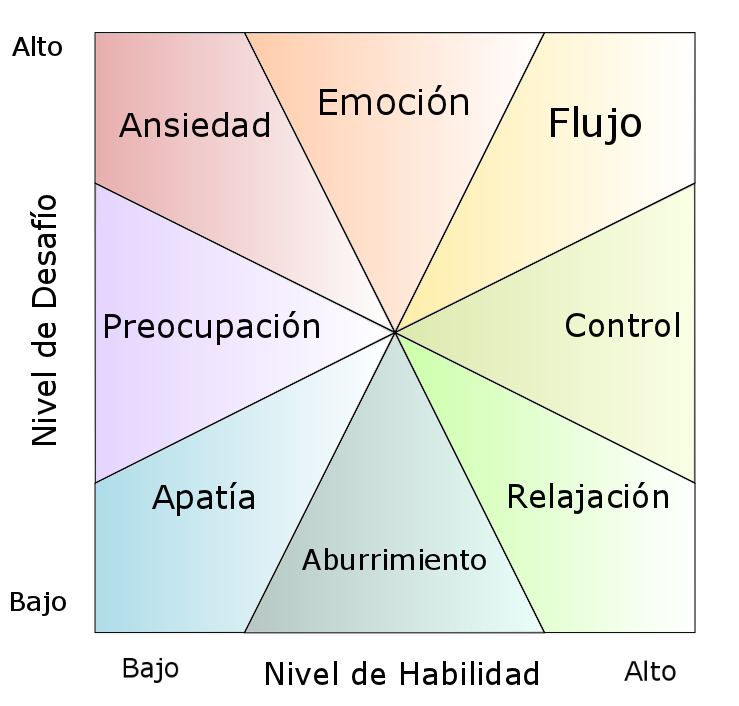
\includegraphics[scale=0.40]{img/Flujo.png}

\small{Fuente: http://www.cluehuntervalencia.com}
\end{center}
\vspace{-0.5cm}
\end{figure}

Csikszentmihalyi entrevistó a jugadores de ajedrez, artistas y deportistas, pero hoy en día, este fenómeno se produce con mucha frecuencia entre los gamers\footnote{Personas con una gran afición por los videojuegos}.
%
La distorsión de la percepción temporal que se produce en el estado de flujo es muy habitual.
%
¿Es posible establecer las condiciones necesarias en un sistema gamificado para que los jugadores entren en estado de flujo?


\subsection{Teoría de la motivación}
\label{SDT}
\label{PosiblesPeligros}
En la Psicología de la Motivación se ha establecido una diferencia entre 2 tipos de motivaciones  \citep{SDT}:  \concept[Motivación\IS Intrínseca]{Motivación intrínseca} -- aquella que depende de los procesos cognitivos internos y está dirigida por el sentido de la autocompetencia, autonomía y relación -- y la \concept[Motivación\IS Extrínseca]{motivación extrínseca} -- aquella que depende de las recompensas que se puedan adquirir con la conducta realizada.
%
Por ejemplo, las actividades autotélicas, mencionadas en la teoría de flujo\crossref{ (ver \ref{autotel})}, necesariamente conllevan una motivación intrínseca.
%
Además de esta diferencia se ha constatado que las conductas motivadas extrínsecamente, sobretodo motivadas con recompensas tangibles, aunque también ocurre con las recompensas verbales, dejan de realizarse cuando desaparece la fuente de motivación, incluso cuando en un momento anterior a la aparición de recompensas la conducta se llevara a cabo motivada intrínsecamente
%
 \citep{ExtrinsicEatsIntrinsic}.

La motivación intrínseca se basa en la \textit{autonomía}, tener la situación bajo control y poder determinar el resultado de las acciones; \textit{competencia} como necesidad de saberse capaz y competente ante los retos y dificultades y \textit{pertenencia} a algo más grande que la propia persona: conectar con otras personas, sentirse parte de la sociedad y compartir los logros.


Es importante conocer esta diferencia a la hora de plantear el objetivo de nuestra gamificación. 
%
Es más sencillo diseñar un sistema de refuerzos basado en el condicionamiento operante, puramente extrínseco que diseñar un sistema que alimente los deseos de autonomía, competencia y pertenencia para fomentar la motivación intrínseca.
%
¿Interesa al diseñador crear un sistema sencillo basado en la motivación extrínseca de los jugadores o, por el contrario, diseñar un sistema más complejo que fomente y haga crecer la motivación intrínseca?



\section{Elementos de la Gamificación}

Tras la exposición de algunas teorías base para la gamificación, se procederá a describir los elementos y las herramientas generales con las que una persona puede diseñar una gamificación para un contexto específico.


\subsection{Pirámide de Werbach}

Los elementos de la Gamificación son los elementos que se encuentran en los juegos, atendiendo a  \cite{werbach2012win} son: dinámicas, mecánicas y componentes, de mayor a menor abstracción.

\concept{Dinámicas} 
%
Las dinámicas son las estructuras implícitas del juego. 
%
Por ejemplo, las reglas serían una manifestación superficial de esa estructura implícita, pero las dinámicas también incluirían manifestaciones conceptuales como podrían ser las restricciones básicas de los juegos, por ejemplo, el respeto a las normas.
%
Se considerarían dinámicas también las emociones, la narrativa, la progresión y las relaciones personales.
%
%\todo{¿Debería incluir alguna definición de los componentes concretos?} 

\concept{Mecánicas} Las mecánicas son los procesos que definen formalmente el contexto y que hacen avanzar la acción. 
%
\label{mecanicas}
%
Por ejemplo, se considerarían mecánicas los retos, la suerte, la competición y la cooperación, el feedback, las recompensas, la adquisición de recursos, las transacciones y los estados de finalización.


\concept{Componentes} Los componentes son las instancias específicas de mecánicas y dinámicas. 
%
Serían componentes los logros, los avatares, los jefes finales\footnote{Batalla muy difícil que tiene lugar al final de cada nivel.}, los combates, el desbloqueo de contenido, los niveles, las misiones, los equipos, las posesiones y el grafo social.
%
Además, hay 3 componentes que merecen una mención específica: los puntos (\textit{points}), las medallas (\textit{badges}) y las clasificaciones (\textit{leaderboards}), comúnmente llamados \gls{PBL}.

Los puntos, por ejemplo, otorgan un feedback acerca del rendimiento y el progreso, es una fuente de datos importante para el diseñador, pueden ligarse con recompensas y se pueden utilizar para determinar los estados de finalización.
%
Las medallas tienen una flexibilidad que permite definir el estilo de un jugador. 
%
Además, tienen un componente social muy importante, ya que muestran el estatus del jugador y son una representación de los logros conseguidos. 
%
También, algunos jugadores se sienten motivados a coleccionarlas.
%
Por último, las clasificaciones o \textit{leaderboards} crean un cierto sentido de competición, en el que los jugadores quieren ascender a puestos más altos de la clasificación, podría ser por el estatus que ofrecen esas posiciones.
%
Se ha estudiado que los \textit{leaderboards} completos desmotivan al 80\% de las personas, debido a la gran brecha que se produce entre los primeros puestos y los últimos.
%
La aproximación más utilizada es diseñar \textit{leaderboards} entre grupos más pequeños de jugadores, por ejemplo, entre los jugadores más cercanos con una puntuación cercana o con sus amigos.



\begin{figure}[hbt]
\begin{center}
\caption{Pirámide de los elementos de Werbach.}
\label{fig::PiramydWerbach}
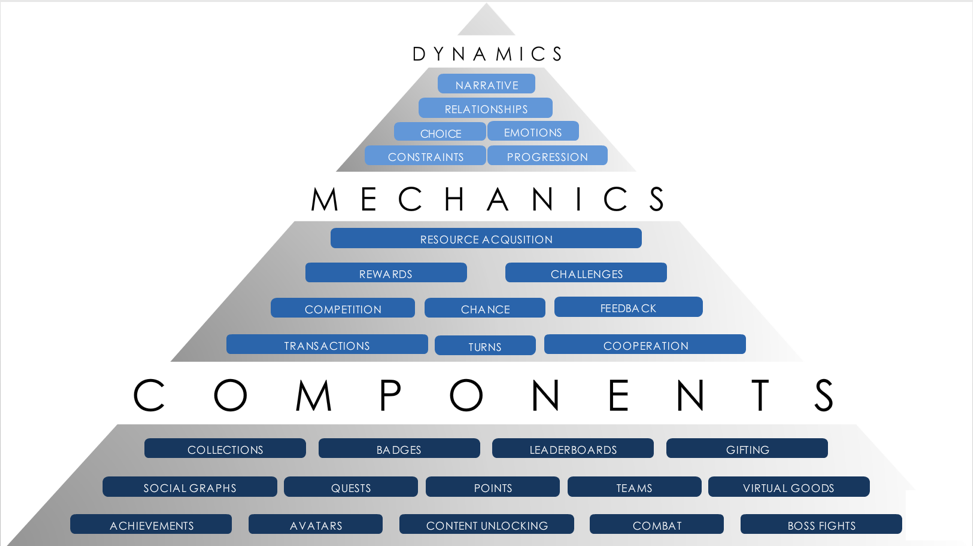
\includegraphics[scale=0.90]{img/Pyramid.png}
\vspace{-0.25cm}
\small{Fuente: \href{http://www.liberty.edu/academics/cafe/index.cfm?id=891255&blogpid=32579&pid=9720}{liberty.edu}.}
\end{center}
\end{figure}
\FloatBarrier



\subsection{Taxonomía de los jugadores}
\label{sec:taxonomy}

\index{Taxonom\'ia de! Bartler}
%
En el proceso de investigación sobre los juegos, sus motivaciones e impactos se ha constatado que no todas las personas responden igual a todos los juegos porque hay tipos de jugadores. 
%
Habiendo distintos tipos de jugadores, no todas las personas responderán por igual a los mismos elementos del juego y habrá elementos más afines a unos tipos de jugadores que a otros. 
%
Por ello, para diseñar correctamente una gamificación es necesario conocer los tipos de jugadores.

Algunas teorías que han tratado de definir una taxonomía de los jugadores, es decir, de clasificar los tipos de jugadores.

 \cite{TypeMUD} estudia a los jugadores de \gls{MUD} según su personalidad y los comportamientos mostrados, según 2 variables: centrados en los jugadores vs centrados el mundo y centrados en la acción y los objetivos del juego vs en la interacción entre jugadores.
%
Estas 2 variables dan lugar a 4 tipos de jugadores, resumido en la imagen \ref{fig::Bartle}:
\begin{itemize}
	\item  \textbf{Triunfadores} (\textit{achievers}): centrados en la acción y en el mundo.
	%
	Tienen un comportamiento individual y quieren llegar a ser los primeros rápidamente.
	

	\item \textbf{Ambiciosos} (\textit{killers}): centrados en la acción y en los jugadores. 
	%
	Estos jugadores buscan las primeras posiciones y además, que los otros jugadores pierdan (de ahí que estén centrados en los jugadores).
	

	\item \textbf{Exploradores} (\textit{explorers}): centrados en la interacción y en el mundo.
	%
	Quieren descubrir y aprender aspectos nuevos del sistema.

	\item \textbf{Sociables} (\textit{socializers}): centrados en la interacción y en los jugadores.
	%
	Juegan para relacionarse con otros jugadores, compartir ideas y experiencias.
\end{itemize}

Se han desarrollado algunos test para clasificar a un jugador en concreto en base a un cuestionario  \cite{Bartletest}.
%
En esta taxonomía no se establece la pertenencia a un tipo único, es decir, una persona puede ser 80\% ambicioso, 15\% triunfador y 5\% explorador.


\begin{figure}[hbt]
\begin{center}
\caption{Taxonomía de los jugadores según Bartle.}
\label{fig::Bartle}
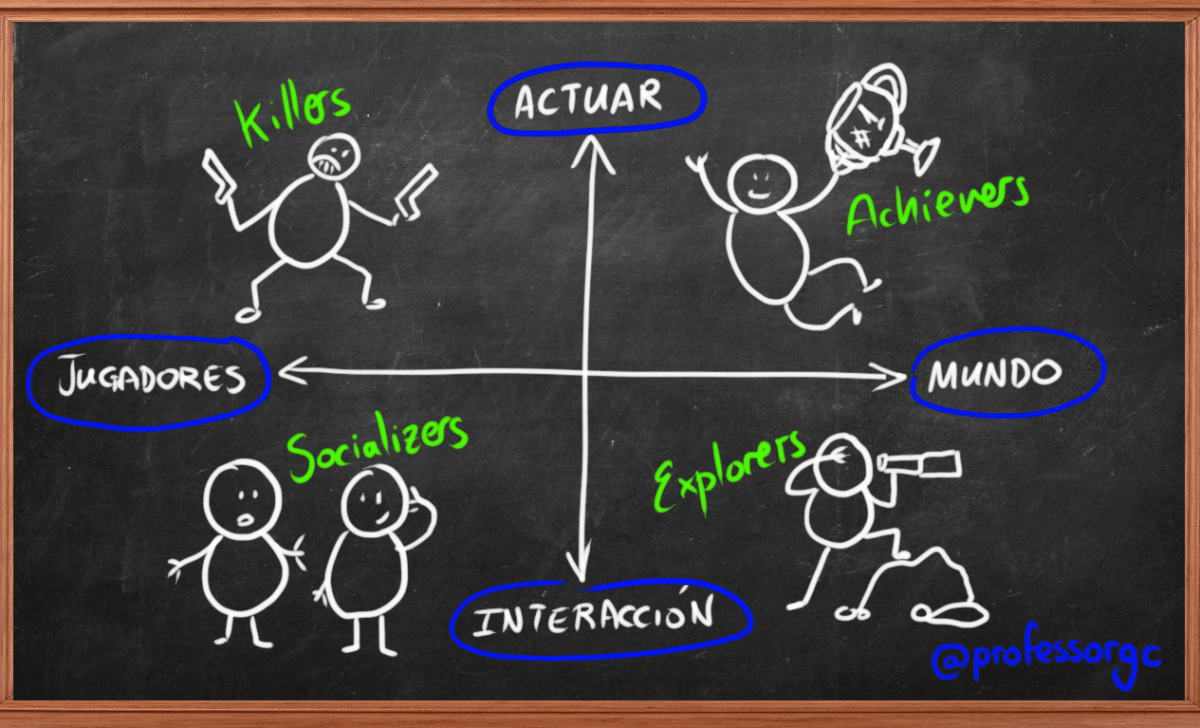
\includegraphics[scale=0.25]{img/Bartle.png}

\vspace{-0.25cm}
\small{Fuente: \url{Creatividadenblanco.com}.}
\end{center}
\end{figure}

Esta clasificación presenta ciertas limitaciones. 
%
La más importante es que se centra en videojuegos \gls{MUD} y, por lo tanto, no es extrapolable a otros juegos; mucho menos a contextos gamificados.
%
Además, el término \textit{killers} en contextos diferentes de videojuegos \gls{MUD} no parece muy adecuado.


\index{Taxonom\'ia de! Amy Jo Kim}
%
Por ello, recurrir a la teoría de  \cite{AmyJoKim}, que se basa en la de Bartle pero la modifica para superar esa limitación.
%
Definen también 4 tipos de jugadores denominados con verbos principales que describen su guía de acción y otros verbos secundarios, como se puede ver en la imagen \ref{fig::AmyJoKim}.
%
La clasificación la hace en base a 2 variables: centrados en el contenido vs centrados en los jugadores y centrados en actuar vs centrados en interactuar.
%
Los jugadores centrados en el contenido y en la actuación serían los competidores (\textbf{compete}), buscando la superación personal.
%
Quienes se centran en el contenido y en la interacción serían los exploradores (\textbf{explore}), buscando el acceso al conocimiento y la información.
%
Los que se centran en los jugadores y en la actuación serían los colaboradores (\textbf{collabore}), buscando formar parte de algo más grande para poder ganar juntos.
%
Por último, las personas que se centran en los jugadores y en la interacción serían los expresivos (\textbf{create}), buscando expresarse, manifestarse y mostrar su creatividad.

\begin{figure}[hbt]
\begin{center}
\caption{Taxonomía de los jugadores según Amy Jo Kim.}
\label{fig::AmyJoKim}
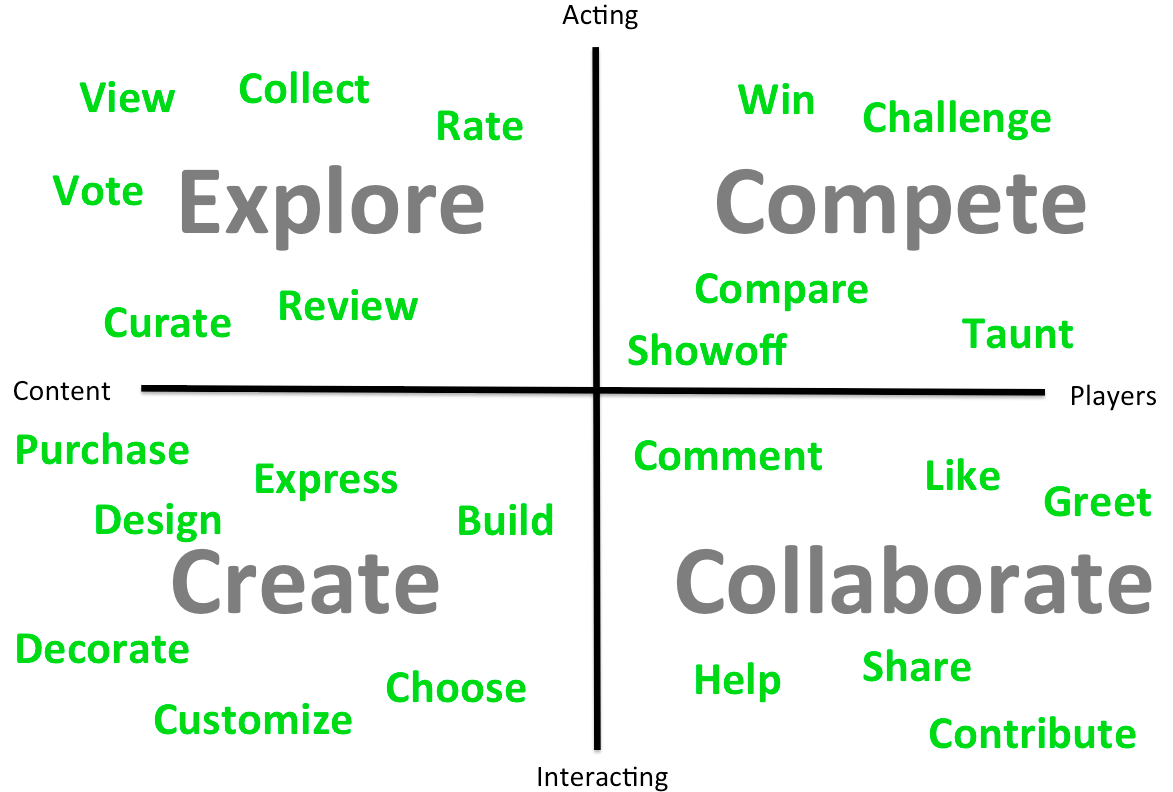
\includegraphics[scale=0.25]{img/AmyJoKim.png}

\vspace{-0.25cm}
\small{Fuente: \url{http://amyjokim.com}.}
\end{center}
\end{figure}


La teoría de Marczewski  \cite{marczewski} es más amplia que las anteriores.
%
Establece más tipos de jugadores, pero además distingue entre jugadores motivados intrínsecamente y extrínsecamente.
%
No sólo eso, sino que los tipos de jugadores motivados extrínsecamente tienen a su vez subgrupos que se parecen a los motivados intrínsecamente, de tal manera que es posible convertir a un jugador motivado extrínsecamente en un jugador motivado intrínsecamente.

En la figura \ref{fig::Marczewski} se puede apreciar el correspondiente esquema de la teoría.
%
En el centro, se encuentra el motivo que guía a cada tipo de jugador. 
%
De estos motivos 4, según  \cite{marczewski} son intrínsecos (Autonomía, Maestría, Relaciones, Propósito\footnote{El único nuevo respecto a la teoría de la auto-determinación  \cite{SDT} es el motivo de \textit{propósito}}) y 2 son extrínsecos: cambio y recompensas.
%
En base a estos 6 motivos, se establecen los 6 tipos de jugadores:
%
Los espíritus libres (\textit{Free spirit}), que son aquellos jugadores que están motivados por la autonomía. Buscan crear y expresarse.
%
Por otro lado, están los triunfadores (\textit{Achiever}), aquellos motivados por la maestría. 
%
Buscan aprender cosas nuevas, mejorar y retos que superar.
%
Quienes están motivados por las relaciones son los socializadores (\textit{Socialiser}).
%
Buscan interactuar con los demás y crear conexiones sociales.
%
El último tipo de jugador motivado intrínsecamente serían los filántropos (\textit{Philantropist}): movidos por el motivo de propósito y significado.
%
Buscan conseguir un propósito que tenga  significado para ellos.
%
Son altruistas y están dispuestos a ayudar a otras personas.
%
Además, se definen los jugadores motivados extrínsecamente, en primer lugar los jugadores (\textit{Player}), motivados por las recompensas. 
%
Harán lo que haga falta para conseguir las recompensas del sistema.
%
A su vez, este tipo de jugador tiene 4 subgrupos: egoísta (\textit{self-esteemer}), consumidor (\textit{consumer}), contacto (\textit{networker}), explotador (\textit{exploitationer}).
%
Para concluir, el último tipo de jugador, también motivado extrínsecamente, sería el perturbador (\textit{Disruptor}) -- aquellos motivados por el cambio. 
%
En general buscan interrumpir el sistema de forma directa o indirectamente (a través de otros usuarios) para forzar el cambio positivo o negativo.
%
Además, este tipo de jugador tiene también 4 subgrupos: influenciador (\textit{influencer}), destructor (\textit{destroyer}), mejorador (\textit{improver}), duelistas (\textit{griefer}).

\begin{figure}[hbtp]
\begin{center}
\index{Taxonom\'ia de! Marczewski}
\caption{Taxonomía de los jugadores según Marczewski.}
\label{fig::Marczewski}
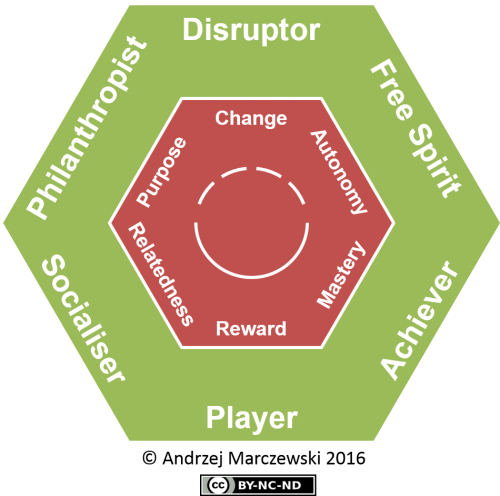
\includegraphics[scale=0.65]{img/Marczewski.jpg}

\vspace{-0.25cm}
\small{Fuente: \url{http://elearningindustry.com}.}
\end{center}
\end{figure}
\FloatBarrier

Como se ha expuesto, esta teoría ofrece un marco de actuación para modificar las motivaciones de los jugadores y transformar a los jugadores extrínsecamente motivados en intrínsecamente motivados.
%
En la figura \ref{fig::MarczewskiEvol} se resume la propuesta de  \cite{marczewski} sobre una posible ruta de evolución de los jugadores para la que, según él, hay cierta evidencia.

\begin{figure}[hbtp]
\begin{center}
\caption{Posible conversión de los jugadores según la taxonomía de Marczewski.}
\label{fig::MarczewskiEvol}
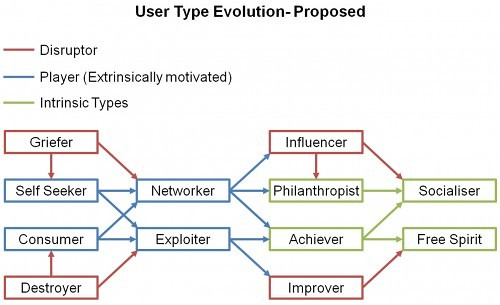
\includegraphics[scale=0.65]{img/evolution.jpg}

\vspace{-0.25cm}
\small{Fuente: \url{http://gamified.uk}.}
\end{center}
\end{figure}
\FloatBarrier





\section{Peligros de la Gamificación}

\subsection{Impacto de la competición en la motivación}


La competición es otra herramienta más a disposición del diseñador, pero es importante tener claro el resultado de algunas investigaciones.
%
Por ejemplo,  \cite{Crawford_CompetitionDef} señala que la competición puede centrar la atención en impedir que el contrincante venza en lugar de centrarse en mejorar y optimizar su propio desempeño.

Otro fenómeno estudiado por  \cite{n-effect} es que el número de competidores y la motivación de los mismos mantienen una relación inversamente proporcional, es decir, cuantos más competidores, menor motivación.

Por último, un estudio llevado a cabo sobre la competición en la educación  \cite{CompetitionInEd} constata que los premios para los ganadores deberían ser de poca importancia o incluso simbólicos para asegurar que el esfuerzo de los estudiantes es intrínseco y no está dirigido por la expectativa del premio.



\subsection{\textit{Pointsification}}

Consiste en la reducción de la gamificación a un simple sistema de puntos en el que se utilizan los aspectos menos esenciales de los juegos y se utilizan como aspectos principales.
%
Los puntos y las medallas en sí no tienen más relación con los juegos que con las páginas web o los programas de fidelización según \cite{Pointsification}.
%
Así, la implementación de una gamificación basada en la mera colección de puntos y medallas no convierte el contexto en divertido ni involucrará a las personas. 
%
Serán necesarios más elementos para llevar a cabo una buena gamificación y no una simple \textit{puntificación}.

\subsection{\textit{Explotationware}}

Un aspecto con el que hay que tener cuidado a la hora de realizar una gamificación es si los futuros jugadores estarían eligiendo libremente participar o no.
%
Si se decidiera utilizar gamificación en una aplicación para fitness, como Nike+, los jugadores que participen lo harán voluntariamente o al menos no obligados por los diseñadores.
%
En cambio, gamificar un entorno laboral o educativo puede resultar más problemático ya que los jugadores pueden perder esa componente de autonomía: no han elegido jugar y por lo tanto su experiencia puede verse perjudicada, fracasando la estrategia.
%
Además, puede no resultar divertido y ser percibido por los trabajadores como una manera de ser controlados y exprimidos en el trabajo.

Un ejemplo de cómo en la gamificación son necesarios muchos más elementos que la competición y las clasificaciones, sería el caso de Disneyland en Anaheim \citep{Explotationware}.
%
En el sótano del hotel, en la lavandería, se colocaron unas pantallas a modo de \textit{leaderboard} con la velocidad de los trabajadores comparados entre ellos.
%
Los trabajadores están listado por el nombre y así, entre compañeros, pueden ver quién es el más rápido haciendo la colada.
%
Lo que podía haberse pensado como una manera de facilitar el trabajo a los operarios, hacerles más agradable el entorno laboral y resolver problemas de eficiencia se había convertido en un desagrado para los trabajadores: éstos se sentían más controlados que antes, ya que sus tiempos estaban continuamente monitorizados y la presión aumentó considerablemente. 
%
Hay trabajadores que cuentan que utilizaban menos el servicio por miedo a aparecer en los últimos puestos de la clasificación.


Con este caso de una gamificación ineficiente, se puede ver que una gamificación mal diseñada no sólo no funciona, sino que es, además, contraproducente. 
%
Una gamificación necesita ser diseñada con cuidado y precisión y eso es lo que va a ser tratado.




\cleardoublepage
%!TEX root = ../TFM.tex


\chapter{Educación gamificada}

A continuación, se estudia cómo se adapta toda la teoría expuesta al ecosistema de un aula.

\coment{Porqué gamificar la educación}

\cite{lee2011gamification} sugieren que el sistema educativo ya contiene elementos de la gamificación, más concretamente \gls{PBL}, ya que los estudiantes realizan unos exámenes para obtener una calificación (puntos) y si se han obtenido más de 5 puntos, se obtiene la medalla de \textit{aprobado}.
%
Incluso, se puede obtener la medalla de \textit{mención de honor} en la evaluación final.
%
Además, encubiertamente se forma un \textit{leaderboard}, ya que los alumnos tienen claro quiénes son los mejores y los peores alumnos (en términos de calificaciones obtenidas).
%
Sin embargo, estos elementos no implican necesariamente motivación por parte de los alumnos.
%
Diseñar una gamificación en un aula puede motivar a los estudiantes, ofrecer a los profesores mejores herramientas para guiar y recompensar a sus estudiantes y enseñar a los estudiantes que la educación puede ser una experiencia divertida  \citep{lee2011gamification}.

Es importante tener en cuenta la teoría de la auto-determinación \crossref{(ver \ref{SDT})} y diseñar una gamificación en el contexto educativo que no debe basarse en una motivación extrínseca, sino fomentar la motivación intrínseca. 
%
De esta manera, los estudiantes podrán desarrollar una mayor capacidad para valorar el aprendizaje y cuando avancen a lo largo del sistema educativo sean capaces de aprovechar contextos educativos no gamificados. 
%
De esta manera, nos interesaría explorar la ruta de evolución \citep{marczewski}  para convertir jugadores extrínsecamente motivados en jugadores intrínsecamente motivados (ver \ref{fig::MarczewskiEvol})


Se ha comentado la existencia de un círculo vicioso (ver figura \ref{fig::circuloVicioso}) y que la variable más influyente en el rechazo hacia las Matemáticas en España es la percepción de la materia como aburrida o divertida.
%
Sería de esperar que, tras lo expuesto, el lector esté de acuerdo en que la Gamificación puede ayudar a modificar esa percepción aprovechando que existen tareas difíciles y divertidas \crossref{(ver \ref{kindsoffun})} además de romper el círculo vicioso por 2 extremos diametralmente opuestos: aburrimiento y desmotivación.

\coment{¿Se puede gamificar la educación? Sí, Cook. 2013}


\section{Proceso de diseño de una Gamificación}

Para diseñar una buena gamificación es necesario seguir un proceso y hay quienes han propuesto un marco con unas pautas para seguir en la tarea. 
%
Como no hay un método consensuado se presentan 2: uno más general  \citep{werbach2012win} y otro más aplicado al contexto educativo  \citep*{kapp2013gamification}.

Werbach define 6 pasos para diseñar una buena gamificación con 6 D's: 
1 - Definir los objetivos de negocio; 2 - Delinear los comportamientos deseados; 3 - Describir a los jugadores; 4 - Diseñar los bucles de actividades; 5 - No olvidarse de la diversión (en inglés: \textit{Don't forget the fun}); 6 - Implementar las herramientas apropiadas (en inglés: \textit{Deploy}).
%
Esta propuesta es demasiado general y no tiene en cuenta algunas características fundamentales del contexto educativo, por ejemplo, la necesidad de un sistema de evaluación.
%
Por ello, una propuesta más centrada en el ámbito educativo puede resultar más útil, sin ignorar por completo la propuesta de Werbach.

La otra propuesta,  \cite{kapp2013gamification}, tiene algunos elementos en común con la de Werbach, pero otros diferentes. 
%
Los autores establecen que se debe pasar por cuatro fases en la gamificación de un contexto educativo. 1 - Responder a las preguntas base; 2 - Responder a las preguntas de práctica; 3 - Diseñar el sistema de valoración y clasificación; 4 - Jugar al juego.

\label{PasosGamificar}
%
Las preguntas base hacen referencia a 5 aspectos: identificar el problema, estudiar los comportamientos existentes, definir los comportamientos deseados, tener claro el objetivo competencial (competencias que los estudiantes necesitan adquirir para que se considerara éxitosa la gamificación) y valorar aspectos que pueden mostrarnos que los alumnos están aprendiendo.
%
Por otro lado, las preguntas de práctica son las preguntas sobre el público objetivo de la gamificación (edad, conocimientos previos, habilidades, tipos de jugadores, etc.), la logística (lugar, momento, tiempo invertido y dinámicas, mecánicas y componentes a utilizar) y las cuestiones técnicas (la disponibilidad de herramientas TIC o no, tanto en el contexto escolar como en el contexto familiar de los estudiantes).
%
En cuanto al sistema de valoración y clasificación es necesario un arduo trabajo.
%
La base logística del sistema tiene que ser completa, es decir, no puede darse el caso en el que no esté especificada la obtención o no de una recompensa o la siguiente meta a alcanzar.
%
Este aspecto es importante, ya que puede haber jugadores que se dediquen a buscar fallos en el sistema y a romperlo para ganar.
%
Por ejemplo, los jugadores de tipo perturbador, según la teoría de  \citet{marczewski}, más concretamente los duelistas dentro de los perturbadores podrían romper la gamificación si encontraran una incompletitud o inconsistencia en el sistema evaluativo.
%
Además, es necesario que el sistema sea justo y permita obtener calificaciones acordes con las competencias y habilidades adquiridas, por ello, las actividades del proyecto, la valoración y el resultado final deben ir unidos.
%
Por último, hay que saber qué acciones pueden realizar los jugadores cuando interactúen (distribuir recursos, coleccionar, cooperar, realizar misiones por otros jugadores, reintentar tareas, etc.). 
%
Es necesario también definir los estados ganadores y el número de oportunidades en cada actividad.

Durante la implementación de la gamificación es importante no perder de vista uno de los puntos que incluye Werbach: No olvidar la diversión.
%
Si un aula gamificada no es divertida para los estudiantes será necesario revisar su diseño y reformarla.


\section{Estado de la Gamificación en la educación en España}

La Gamificación como metodología docente está en auge. 
%
Una prueba de ello es el \gls{MOOC} del \gls{INTEF} que tuvo su primera edición en Octubre de 2016.
%
Otra prueba es la iniciativa: \textit{Gamifica tu aula}, un grupo de docentes en España desde infantil hasta el ámbito universitario que emplean esta metodología y utilizan una web \footnote{\url{http://gamificatuaula.wixsite.com/ahora}} con para darse a conocer, compartir recursos y ayudar a docentes que se quieran iniciar en el campo de la gamificación.
%
Tienen también un perfil en twitter\footnote{\href{https://twitter.com/gamificatuaula}{@gamificatuaula}} con casi 3000 seguidores, con el que intentan dar difusión a sus propuestas y ser contactados.
%
Entre estos profesores se encuentra Javier Espinosa Gallardo, Premio Innovación SIMO 2015 y Premio Nacional de Educación 2015, ambos premios por su proyecto de gamificación interdisciplinar \href{http://jespinosag.wixsite.com/classofclans}{\textit{Class of clans}}.

Al presentarse en la web, dicen:
%
"Tenemos la clara convicción, a partir de experimentar en nuestras aulas, de que [la Gamificación] mejora los procesos de aprendizaje, la motivación, el desarrollo de la inteligencia emocional y la adquisición de habilidades como la cooperación o la resiliencia, entre otras." 
%
y esta convicción quieren difundirla y "colonizar".
%
Consideran además que ’A gamificar se aprende gamificando‘.

Se observa que no es novedad absoluta plantear la Gamificación en la educación España, pues ya se está utilizando.
%
Sin embargo, la tasa adopción por parte de los docentes es escasa, ya que el número de centros y de profesores es inmensamente mayor que el número de profesores empleando la Gamificación.
%
En parte puede deberse al desconocimiento por parte de los docentes de esta metodología o al sobresfuerzo que puede ser necesario para diseñar una buena Gamificación.

\section{La Gamificación en la enseñanza de Matemáticas}

Lo ideal sería poder diseñar gamificaciones interdisciplinares por varias razones.
%
La primera y más importante, por la necesidad y beneficios de un sistema educativo menos compartimentado. 
%
Los problemas globales han aumentado en complejidad y conectividad (crisis de refugiados, del agua, cambio climático, crecimiento poblacional, etc.), lo que obliga a enfocarlos como complejos, inseparables y retroalimentados, desde una perspectiva interdisciplinar \citep{Interdiscip}
%
Por otro lado, la duplicidad de esfuerzos que supondría realizar gamificaciones distintas para aulas distintas sería un disparate.

Sin embargo, en la realidad los escenarios ideales no se alcanzan a la primera.
%
Además, las experiencias de gamificación interdisciplinar según \textit{gamificatuaula.com} han surgido de una gamificación monodisciplinar que ha ido contagiando e involucrando a otros docentes.


Por otro lado, no todas las mecánicas, dinámicas y componentes de la Gamificación se pueden aplicar por igual a las diferentes asignaturas.
%
Por ejemplo, \cite{ClassAVideogame} diseñó una gamificación en su aula de biología en la que los distintos niveles eran distintas fases en la investigación de un virus para sobrevivir una pandemia.
%
Esos niveles se ajustan relativamente bien al curriculum de la asignatura y al temario a impartir.
%
Otro ejemplo sería una gamificación diseñada por Javier Espinosa, en la que los distintos niveles eran especies animales, de menor a mayor complejidad.
%
En asignatura como Historia y Geografía, los niveles se pueden diseñar como ascensos dentro de un sistema feudal \citep{Feudal}.

En Matemáticas esa herramienta es difícil de aplicar con un sentido tan pleno.
%
Sin embargo, hay otros elementos que, por las características propias de cada asignatura, son muy útiles.
%
Las Matemáticas permiten plantear retos (ejercicios y problemas) de muy diversa dificultad: se puede plantear un reto de comienzo de la clase, el reto del día, el reto de la semana, etc. con la dificultad que en cada momento sea necesaria.
%
Además, se pueden plantear problemas contextualizados en la narración de la gamificación, por ejemplo, de geometría.
%
Si se utilizara una narrativa sobre la sociedad de la Grecia antigua, como el proyecto Helade (2015/2016), los problemas a los que se enfrentaban Pitágoras y Tales se pueden contextualizar en esa narrativa a la perfección.


Independientemente de la narrativa que se utilice hay una gran cantidad de elementos disponibles a utilizar en la gamificación. 
%
Por las características de las Matemáticas algunos elementos que podrían tener más sentido serían las misiones y los retos, los jefes finales y el desbloqueo de herramientas, pudiendo desbloquear teoremas y resultados para resolver problemas más difíciles.


%%%%%%%%%%%%%%%%%%%%%%%%%%%%%%%%%%%%%%%%%%%%%%%%%%%%%%%%%%%%%%%%%%%%%%%%%%%%%%%%
%%%%%%%%%%%%%%%%%%%%%%%%%%%%%%%%%%%%%%%%%%%%%%%%%%%%%%%%%%%%%%%%%%%%%%%%%%%%%%%%
% DISEÑO E IMPLEMENTACIÓN %
%%%%%%%%%%%%%%%%%%%%%%%%%%%%%%%%%%%%%%%%%%%%%%%%%%%%%%%%%%%%%%%%%%%%%%%%%%%%%%%%

\cleardoublepage
%!TEX root = ../TFM.tex

\newcommand{\arab}{al-Karaji}
\newcommand{\Arab}{Al-Karaji}
\newcommand{\logro}[2]{\labeltext{#1\xspace}{logro::#2} #1\xspace}


\chapter{Gamificar las Matemáticas}

%Lo que debes reflfejar en este capítulo es cómo lo has hecho, cual es tu objetivo, como organizas el aula, como lo evaluas y qué resultados obtienes.

%Una vez explicitados los fundamentos sobre los que basamos nuestra propuesta metodológica, procedemos a su descripción.

%\section{Objetivos}

El principal objetivo es ofrecer una propuesta de trabajo que suponga una innovación y una mejora en el actual sistema educativo.
%
Para ello, ofrecemos una concreción de la metodología estudiada con la que desarrollar una Unidad Didáctica.
% 
Por otro lado, se espera que esta propuesta suponga para los alumnos un proceso de enseñanza-aprendizaje en el que puedan adquirir las competencias y aprendizajes necesarios de una manera más profunda, duradera y entretenida.

%Para ello, se desarrollará la propuesta y después se ofrecerá un marco de investigación \crossref{(ver \ref{evalGami})} para evaluar si esta propuesta metodológica supone realmente una innovación y una mejora.

\section{Diseño de la gamificación}

Se ha tratado, en términos generales, la propuesta para diseñar una gamificación de \cite{kapp2013gamification}. 
%
Se va a utilizar esa propuesta para guiar el proceso de diseño de la gamificación. 
%
Para ello, se irán recorriendo las etapas propuestas.

El primer paso consiste en estudiar el problema que se quiere resolver. 
%
Éste ha sido tratado con amplitud anteriormente\crossref{(ver sección \ref{chap:intro})}, estudiando los comportamientos existentes. 
%
Por otro lado, el comportamiento deseado sería que los estudiantes estuvieran más motivados y comprometidos con la asignatura, dispuestos a trabajar activamente en clase y trabajaran en casa.
%
Además, el objetivo competencial está definido por el \bocm y se detallará más adelante\crossref{(ver \ref{tbl:Matrizdetodo})}.
%
El último aspecto de las preguntas base es la valoración de los aspectos que puedan darnos retroalimentación sobre el proceso.
%
La manera en la que se va a conseguir eso es mediante el diseño de un itinerario de logros y puntos que los alumnos van recorriendo.
%
De esta manera se puede anticipar fácilmente si hay algún alumno rezagado simplemente observando los logros adquiridos y los puntos.
%
No obstante, en cada sesión y tarea se especificará un mínimo a alcanzar por parte de los alumnos.

En el segundo paso se trabajan las preguntas prácticas.
%
El público objetivo de la gamificación son alumnos de secundaria del sistema educativo español. 
%
Debido a que esta gamificación no se plantea para ser aplicada en un centro en concreto, no se pueden determinar con exactitud los conocimientos previos y habilidades ni los tipos de jugadores concretos a los que esta propuesta se dirige.
%
No obstante, en este trabajo se han tratado los tipos de jugadores \crossref{(ver \ref{sec:taxonomy})} para que el docente, en el momento de implantación de esta gamificación pueda definir los tipos de jugadores concretos a quienes se dirige la gamificación.
%
Por otro lado, la definición logística y técnica de la gamificación se encuentra especificado a lo largo de la descripción de la unidad didáctica \crossref{(ver sección \ref{sec:UD})}, teniendo en cuenta los recursos existentes y las habilidades del docente.

Asimismo, el sistema de valoración también está incluido en la unidad didáctica, anticipando durante el diseño los posibles fallos del sistema para conseguir una evaluación lo más justa posible.

El último paso de la propuesta de \cite{kapp2013gamification} sería la puesta en marcha del sistema. 
%
Desafortunadamente, esta gamificación no ha sido llevada al aula todavía.

\subsection{Marco legal de aplicación}

La \lomce establece que: "Necesitamos propiciar las condiciones que permitan el oportuno cambio metodológico, de forma que el alumnado sea un elemento activo en el proceso de aprendizaje" 
%
En este sentido, nuestra propuesta metodológica se apoya en las indicaciones establecidas por la \lomce para el ejercicio de la labor docente.

La \lomce establece condiciones generales que son concretadas por el \boe, estableciendo los contenidos que se deben tratar en cada curso.
%
Después, corresponde a cada Administración la elaboración del currículo básico para su comunidad autónoma.
%
En este caso, recurrimos al \bocm.


\subsection{Elección del curso para Gamificar}

El curso elegido para desarrollar la propuesta es Matemáticas Orientadas a las Ciencias Académicas de 3º de ESO por ser 3º de ESO el curso en el que se constata que se ha producido un aumento del rechazo hacia las Matemáticas \crossref{(ver sección \ref{sec:estudioNacional})} 
%
Además, es también el curso en el que la percepción de la asignatura como divertida menor en este curso (40,46\% en 3º de ESO frente a 54,46\% en Bachillerato y 68,51\% en 1º de ESO) \cite{ActitudesHaciaMates}.

Dentro del curso se ha elegido desarrollar una unidad didáctica sobre los polinomios porque es el primer curso en el que se tratan los polinomios y su mal aprendizaje puede lastrar al alumno hasta los primeros cursos universitarios.
%
La factorización de polinomios, por ejemplo, es un recurso importante en la diagonalización de matrices, contenido fundamental en Álgebra de cualquier grado en Ingeniería o Administración y Dirección de Empresas.
%
Si en este curso se consigue un aprendizaje consolidado y duradero, los estudiantes podrán desempeñar y aprovechar mejor los cursos venideros.


\section{Unidad didáctica gamificada}

\label{sec:UD}
%
Esta unidad didáctica pertenece a la asignatura Matemáticas Orientadas a las Ciencias Académicas de 3º ESO. 
%
Los contenidos de la asignatura, definidos en el \boe y matizados por el \bocm, se dividen en 5 bloques:
1) Procesos métodos y actitudes en las matemáticas. 
2) Números y álgebra: Números racionales, números decimales, polinomios, sucesiones, ecuaciones y sistemas.
3) Geometría: geometría plana, geometría del espacio, globo terráqueo, uso de herramientas tecnológicas.
4) Funciones.
5) Estadística y probabilidad.

Esta unidad didáctica pertenece al bloque de Números y Álgebra para tratar el punto 6 de los contenidos del bloque 2 según el \bocm: \comillas{Polinomios. Expresiones algebraicas.}
%
Este punto incluye:
%
\comillas{Transformación de expresiones algebraicas, igualdades notables, operaciones elementales con polinomios. 
%
Ecuaciones de primer y segundo grado con una incógnita y resolución por el método algebraico y gráfico de ecuaciones de primer y segundo grado.}
%
Más adelante, en la tabla \ref{tbl:Matrizdetodo} se expondrán más claramente los Contenidos, Criterios de Evaluación y \eaes pertinentes.

Esta unidad didáctica desarrollará todo lo relativo a polinomios y su manejo, excluyendo las ecuaciones y sistemas de ecuaciones que corresponderán a otra unidad didáctica diferente.

\subsection{Conocimientos previos}

Es fundamental que los alumnos recuerden las propiedades de las potencias de exponentes naturales con las que llevan trabajando al menos 2 cursos.
%
Asimismo, sería conveniente que los estudiantes recordaran qué es una expresión algebraica y cómo calcular su valor numérico.
%
No obstante, esto último será repasado en el desarrollo de esta unidad didáctica para corregir posibles desequilibrios entre los niveles de los alumnos.



\subsection{Contenidos y Estándares de Aprendizaje Evaluables}

En la tabla \ref{tbl:Matrizdetodo} se encuentran resumidos los Contenidos, Criterios de Evaluación y  Estándares de Aprendizaje Evaluables de la unidad didáctica desarrollada.

\begin{table}[hbt]
\centering
\caption{Matriz de Contenidos, Criterios de Evaluación y  Estándares de Aprendizaje Evaluables de la unidad didáctica}
\label{tbl:Matrizdetodo}
\begin{tabular}{|p{0.24\linewidth}|p{0.3\linewidth}|p{0.42\linewidth}|}
\hline
 \multicolumn{1}{|c|}{Contenidos} & \multicolumn{1}{|c|}{Criterios de Evaluación} & \multicolumn{1}{c|}{\eaes}
\\\hline

\mylabel{C261}{Cont. 2.6.1} Transformación de expresiones algebraicas. 
&
\multirow{3}{\linewidth}{\mylabel{CE23}{C.E. 2.3} Utilizar el lenguaje algebraico para expresar una propiedad o relación dada mediante un enunciado, extrayendo la información relevante y transformándola.\vfill}
& 
\mylabel{EAE3.1}{E.A.E. 3.1}: Realiza operaciones con polinomios y los utiliza en ejemplos de la vida cotidiana.
\\\cline{1-1} \cline{3-3} 

\mylabel{C262}{Cont. 2.6.2} Igualdades notables. 
&
& 
\mylabel{EAE3.2}{E.A.E. 3.2}: Conoce y utiliza las identidades notables correspondientes al cuadrado de un binomio y una suma por diferencia, y las aplica en un contexto adecuado. 
\\\cline{1-1} \cline{3-3} 

\mylabel{C263}{Cont. 2.6.3} Operaciones elementales con polinomios. 
&
&
\mylabel{EAE3.3}{E.A.E. 3.3}: Factoriza polinomios de grado 4 con raíces enteras mediante el uso combinado de la regla de Ruffini, identidades notables y extracción del factor común.
\\\hline
\end{tabular}
\end{table}
\FloatBarrier

\subsection{Metodología:}

La metodología principal aplicada en esta unidad didáctica será la gamificación.
%
Ésta se apoyará de otras estrategias metodológicas como la colaboración y el trabajo en grupo para la realización de algunos trabajos concretos, el trabajo autónomo y la exposición en la pizarra o con proyecciones por parte del docente.

Con esta metodología específica se pretende aportar las condiciones necesarias para que el aprendizaje de los alumnos sea significativo, funcional y duradero.
%
También aporta un enfoque lúdico y emocionante al aprendizaje ya que, como es bien sabido, sin emoción no tiene lugar el aprendizaje.
%
Además, esta elección metodológica permite hacer protagonista al alumno durante el proceso logrando que se involucre activamente en el proceso de enseñanza-aprendizaje.
%
%Por último es una metodología tremendamente flexible que permite sinergias con otras metodologías como el aprendizaje cooperativo y la clase invertida.


Los elementos de la gamificación utilizados son la narrativa, los logros y medallas, los puntos de reputación, que a su vez sirven para comprar bienes reales en una economía de fichas, los retos que pueden ser retomados varias veces y un reto complicado al final de la Unidad Didáctica a modo de jefe final.


Otro aspecto de la estrategia metodológica es la utilización de herramientas \gls{TIC}, sobre las que la \lomce establece que \comillas{serán una pieza fundamental para producir el cambio metodológico que lleve
a conseguir el objetivo de mejora de la calidad educativa.}
%
Los ejercicios de trabajo autónomo por parte del estudiante en horario no lectivo serán realizados en una plataforma online (\textit{edmodo}) de tal manera que el estudiante pueda recibir feedback inmediato de su desempeño.
%
Salvo que se especifique lo contrario, no es relevante el tiempo empleado en la resolución de estos ejercicios sino su resolución satisfactoria o insatisfactoria.
%
Se fomentará la corrección en las respuestas más que la rapidez con un bonus acumulativo por respuestas correctas, además de ofrecer la posibilidad de retomar el ejercicio un número de veces determinado, para facilitar el aprendizaje a partir de los errores y los fallos.
%
Estos parámetros dependerán de cada set de ejercicios y se especificarán pertinentemente.

En algunos momentos se trabajará por grupos.
%
Los grupos serán de 4 personas y se buscarán que estén equilibrados.
%
Se utilizarán las notas de Matemáticas del año pasado para equilibrar la competencia matemática de los distintos grupos y el conocimiento del docente de los alumnos para crear grupos que puedan funcionar de la mejor manera posible, separando parejas, mejores amigos y enemigos.
%
\label{grupos}
%
Los grupos se harán el primer día y siempre que se trabaje en grupos, será en estos grupos.

En esta unidad didáctica se está priorizando el aprendizaje activo de los contenidos y competencias otorgando menos importancia a otras habilidades transversales y necesarias como tomar apuntes y notas en clase. 
%
Esta competencia es muy útil (aunque cada vez más en desuso) y se priorizará en otras unidades didácticas del curso. 
%
Se ofrecerá a los alumnos un libro de texto de apoyo para que puedan consultar cuando necesiten cualquier aspecto teórico.
%
Para esta unidad didáctica, al no estar suscrita a ningún centro utilizaremos un material didáctico elaborado por \citeauthor{MareaVerde} en \citeyear{MareaVerde} en el movimiento de la Marea Verde \citep{MareaVerde}.


\subsubsection{Concreciones metodológicas}

La narrativa de la Gamificación consistirá en la simulación de un instituto de investigación histórica.
%
Los alumnos son los historiadores con una mayor competencia matemática de Europa y se necesita su ayuda para encontrar un tesoro árabe que se escondió en Madrid en 1083, justo antes de la reconquista cristiana.

Se han encontrado una serie de documentos que no se ha conseguido descifrar en su totalidad y se cree que los alumnos van a ser capaces de resolverlo.
%
%
Este documento utiliza las matemáticas de Abu Bekr ibn Muhammad ibn al-Husayn al-Karaji, el primero en definir los monomios $x$,$x^2$... y proporcionar reglas para su producto, es decir, el primero en definir las bases del álgebra\citep{MatArabe}.
%
Para poder resolver el enigma será necesario que aprendamos las matemáticas que se utilizaban en Al-Ándalus.

Será necesario que en su cuaderno incorporen un diario del investigador, en el que ir tomando notas de lo que les resulte importante, dejando constancia de los avances que van realizando, etc.
%
En cada clase se irán obteniendo partes de las coordenadas geográficas de un lugar de Madrid y se irán aprendiendo herramientas para resolver el problema.

%%%%%%%%%%%%% \todo{Definir el lugar donde está el tesoro}

%%%%%%%%%%%%%%%%%%%%%%%%%%%%%%%%%%%%%%%%%%%%%%%%%%%%%%%%%%%%%%%%%%%%%%%%%%
%%%%%%%%%%%%%%%%%%%%%%%%%%%%%%%%%%%%%%%%%%%%%%%%%%%%%%%%%%%%%%%%%%%%%%%%%%
%%%%%%%%%%%%%%%%%%%%%%%%%%%%%%%%%%%%%%%%%%%%%%%%%%%%%%%%%%%%%%%%%%%%%%%%%%
%%%%%%%%%%%%%%%            TEMPORALIZACIÓN           %%%%%%%%%%%%%%%%%%%%%
%%%%%%%%%%%%%%%%%%%%%%%%%%%%%%%%%%%%%%%%%%%%%%%%%%%%%%%%%%%%%%%%%%%%%%%%%%
%%%%%%%%%%%%%%%%%%%%%%%%%%%%%%%%%%%%%%%%%%%%%%%%%%%%%%%%%%%%%%%%%%%%%%%%%%
%%%%%%%%%%%%%%%%%%%%%%%%%%%%%%%%%%%%%%%%%%%%%%%%%%%%%%%%%%%%%%%%%%%%%%%%%%
%%%%%%%%%%%%%%%%%%%%%%%%%%%%%%%%%%%%%%%%%%%%%%%%%%%%%%%%%%%%%%%%%%%%%%%%%%


\subsection{Temporalización}

La unidad didáctica se divide en 10 sesiones.
%
Para una explicación más desarrollada de las sesiones, ver el apéndice \ref{app:todo}.


\label{ResumenSesion1}
%
La primera sesión es introductoria.
%
Se explicará la gamificación y su narrativa. 
%
Además, se crearán los grupos de trabajo para cuando sea necesario trabajar en equipo.
%
Hasta la finalización de la sesión se realizará un \textit{Kahoot} con el que repasar contenidos y conceptos que deberían saber de años anteriores.

\label{ResumenSesion2}
%
En la segunda sesión se trabajará la introducción a los polinomios, dentro de la narrativa de la gamificación. 
%
Los alumnos trabajaran autónomamente en un reto, cuya correcta resolución otorgará el logro \ref{logro::investigador_apto}.
%
En caso de que el trabajo en clase se haya desarrollado satisfactoriamente y todos los alumnos hayan conseguido descifrar el acertijo, se propondrá un pequeño test online (incluido en el anexo \ref{test:ses1}).
%
Excepcionalmente, en el caso de que el trabajo haya resultado muy complicado a los alumnos se podría emplear una sesión más en realizar los ejercicios del test en clase, con las explicaciones pertinentes del profesor.

\label{ResumenSesion3}
%
En la tercera sesión se procederá a una exposición por parte del profesor sobre la multiplicación de polinomios y los alumnos se enfrentarán a otro reto, esta vez por grupos debido al incremento de dificultad.
%
Para trabajar en casa se les propondrán varios ejercicios en la plataforma online de los que tendrán que seleccionar un número determinado. 
%
En principio serían 3, pero este valor puede ser modificado dependiendo del desempeño de los alumnos durante la sesión.
%
Cada ejercicio tendrá asociado una puntuación: los ejercicios más difíciles otorgan más puntos, los ejercicios más fáciles, menos puntos.

\label{ResumenSesion4}
%
La siguiente sesión se desarrollará con un esquema muy parecido, salvo que el contenido a trabajar será la división de polinomios.
%
Sin embargo, el trabajo en casa de esta sesión no será para practicar habilidades matemáticas sino para involucrarse más con la narrativa de la gamificación.

\label{ResumenSesion5}
%
En la quinta sesión se pondrá en marcha la posibilidad de conseguir un logro nuevo, \ref{logro::avizor}, por la identificación y resolución de una identidad notable.
%
La sesión transcurrirá con explicaciones por parte del profesor y ejemplos resueltos en la pizarra (en los que los alumnos podrán obtener subniveles del logro), seguidos de trabajo autónomo por parte del alumno.
%
No se propone trabajo para realizar extraescolarmente.

\label{ResumenSesion6}
%
La siguiente sesión se dividirá en 2 partes. 
%
Se explicará el algoritmo de Ruffini para dividir y se les propondrá el mismo desafío que en la sesión 3, el de las divisiones.
%
De esta manera podrán comprobar el potencial del algoritmo, ya que deberían emplear bastante menos tiempo en su resolución.
%
Una vez entendido y practicado Ruffini como algoritmo de división, se procederá a explicar cómo se puede factorizar un polinomio utilizando este algoritmo y se realizarán ejercicios prácticos.
%
Para trabajar en casa se propondrán ejercicios en \textit{edmodo} con el esquema utilizado anteriormente.
%
En estos deberes se incorporará un vídeo con la explicación teórica sobre la factorización de polinomios con coeficiente principal distinto de 1.


\label{ResumenSesion7}
%
\label{ResumenSesion8}
%
En las siguientes 2 sesiones se propondrá un desafío complicado que implica aplicar con soltura todos los conocimientos aprendidos además de seguir aplicando conocimiento de años anteriores.
%
En la primera sesión se trabajará individualmente (cada miembro del equipo tendrá una ficha ligeramente diferente) y la segunda se trabajará cooperativamente.
%
Para la segunda sesión será necesario que los alumnos hayan finalizado con éxito sus partes individuales, ya que el equipo necesitará los resultados obtenidos en la parte individual.

\label{ResumenSesion9}
%
En la última sesión, no necesariamente la sesión siguiente, tendrá lugar el examen de la unidad.



\subsection{Recursos}

\subsubsection{Recopilación de los elementos de la gamificación }

Los recursos de la gamificación utilizados se encuentran descritos en la tabla \ref{Gamify:resumen}.

\begin{table}
\centering
\caption{Recopilación de los elementos de la gamificación utilizados}
\label{Gamify:resumen}
\begin{tabular}{|m{0.06\linewidth}|m{0.35\linewidth}|m{0.42\linewidth}|}
\hline
ID & Nombre & Descripción\\\hline
EG1\labeltext{EG1}{puntos} & Puntos de reputación & Todos los puntos que se obtienen son de reputación.
%
El profesor podrá otorgar puntos de reputación a los alumnos por hacer preguntas interesantes o ayudarse entre ellos.
\\\hline
EG2\labeltext{EG2}{apto} & Logro \ref{logro::investigador_apto} &\\\hline
EG3\labeltext{EG3}{nato} & Logro \ref{logro::investigador_nato} &\\\hline
EG4\labeltext{EG4}{comp} & Logro \ref{logro::investigador_comprometido} & Niveles.\\\hline
EG5\labeltext{EG5}{avizor} & Logro \ref{logro::avizor} & Niveles.\\\hline
EG6\labeltext{EG6}{context} & Logro \ref{logro::contextualizador} & Niveles.\\\hline
EG7\labeltext{EG7}{narrativa} & Narrativa & Los alumnos son investigadores de unos manuscritos árabes.\\\hline
EG8\labeltext{EG8}{explorador} & Medalla \logro{Explorador}{explorador} & Obtenible por hacerse la foto en el lugar del tesoro.\\\hline
EG9\labeltext{EG9}{eleccion} & Elección & Posibilidad de elección de los deberes a realizad (Mecánica de la gamificación). \\\hline
EG10\labeltext{EG10}{feedback} & Retroalimentación inmediata & Utilización de una herramienta online para aportar retroalimentación inmediata a los alumnos al realizar los deberes \\\hline
EG11\labeltext{EG11}{fichas} & Economía de fichas & Tienda en la que poder comprar ciertos privilegios con los puntos obtenidos a lo largo de las sesiones. Descritos en \ref{tbl:tienda}. \\\hline
\end{tabular}
\end{table}
\FloatBarrier

\todo{Definir puntos de la tienda}

\begin{table}[hptb]
\centering
\caption{Artículos de la economía de fichas}
\label{tbl:tienda}
\begin{tabular}{|m{0.15\linewidth}|m{0.2\linewidth}|m{0.6\linewidth}|}
\hline
Puntos & Nombre & Descripción \\ \hline
$n$ & ExtraQuizz	& Aumentar en 1 el número de ejercicios que se pueden hacer en \textit{edmodo} para ganar puntos.\\\hline
$x^2·m$ & TeacherQuizz & $x$ preguntas directas (de sí o no) y precisas\footnotemark al docente en el examen\\\hline
$t$ & Miniatura algebraica & Una botella de Klein impresa en 3D \citep{Klein} \\\hline
$s$ & Bonus x2 & Obtención de un bonus duplicador de puntos para una sesión.\\\hline
%$r$ &  &  \\\hline
\end{tabular}
\footnotetext{Preguntas del tipo: ¿Este ejercicio está bien? es demasiado ambigua y no sería válida. Preguntas como: ¿Con el ejercicio así obtendría la máxima puntuación? sí sería válida.
%
El grado de precisión de una pregunta será competencia única del docente en el momento del examen.}
\end{table}
\FloatBarrier

\subsection{Evaluación}

\label{eval}
%
La evaluación que se propone para esta unidad didáctica es a través de un examen incluido en \ref{examen} con la ponderación que estuviera establecida en la \gls{PDA} y el trabajo de clase, que se medirá mediante los puntos y medallas obtenidos por cada alumno.

Para establecer ponderación de las medallas y de los puntos de reputación para obtener la calificación del trabajo de clase se propone el siguiente sistema:
%
de los 10 puntos de actitud y trabajo en clase, hasta un máximo de 5 puntos se podrán obtener mediante logros, otorgando cada logro un punto\footnote{2 niveles de un mismo logro otorgarán 2 puntos} y hasta un máximo de 5 puntos se podrán obtener mediante puntos de reputación, mediante una regla de 3, correspondiendo 5 puntos con ¿100?\todo{por definir} puntos de reputación y 0 puntos con 0 puntos de reputación.


La evaluación a través de un examen tiene varias ventajas:
%
la primera es la facilidad de la incorporación de esta unidad didáctica en un curso que ya funcione con metodologías tradicionales. 
%
No hace falta modificar los criterios de evaluación que se hubieran establecido para evaluar a los alumnos.
%
Además, permite y facilita la experimentación.
%
Se pueden comparar los resultados del aprendizaje mediante un examen en un curso que ha participado en la gamificación frente a un curso que haya recibido las sesiones mediante otras metodologías.
%
En el caso de que esta estrategia metodológica fuese adoptada por un único docente en un departamento, la posible experimentación permitiría iniciar un diálogo y debate sobre la incorporación de la gamificación por parte de otros docentes, incluso en otros cursos.

Dicho lo cual, sería injusto no comentar que la evaluación mediante un examen no es la mejor manera de realizar una evaluación justa que asegure la adquisición de las competencias y el aprendizaje duradero los contenidos.
%
Se podrían utilizar rúbricas por ejemplo, que permitirían una evaluación mucho más exhaustiva y personalizada.
%
Sin embargo, se ha preferido optar por el examen por todo lo comentado anteriormente.



%%%%%%%%%%%%%%%%%%%%%%%%%%%%%%%%%%%%%%%%%%%%%%%%%%%%%%%%%%%%%%%%%%%%%%%%
%%%%%%%%%%%%%%%%%%%%%%%%%%%%%%%%%%%%%%%%%%%%%%%%%%%%%%%%%%%%%%%%%%%%%%%%
%%%%%%%%%%%%%%%%%%%%%%%%%%%%%%%%%%%%%%%%%%%%%%%%%%%%%%%%%%%%%%%%%%%%%%%%
%%%%%%%%%%%%%%%%%%%%%%%%%%%%%%%%%%%%%%%%%%%%%%%%%%%%%%%%%%%%%%%%%%%%%%%%
%%%%%%%%%%%%%%%%%%%%%%%%%%%%%%%%%%%%%%%%%%%%%%%%%%%%%%%%%%%%%%%%%%%%%%%%
%%%%%%%%%%%%%%%%%%%%%%%%%%%%%%%%%%%%%%%%%%%%%%%%%%%%%%%%%%%%%%%%%%%%%%%%
%%%%%%%%%%%%%%%%%%%%%%%%%%%%%%%%%%%%%%%%%%%%%%%%%%%%%%%%%%%%%%%%%%%%%%%%
%%%%%%%%%%%%%%%%%%%%%%%%%%%%%%%%%%%%%%%%%%%%%%%%%%%%%%%%%%%%%%%%%%%%%%%%
%%%%%%%%%%%%%%%%%%%%%%%%%%%%%%%%%%%%%%%%%%%%%%%%%%%%%%%%%%%%%%%%%%%%%%%%
%%%%%%%%%%%%%%%%%%%%%%%%%%%%%%%%%%%%%%%%%%%%%%%%%%%%%%%%%%%%%%%%%%%%%%%%
%%%%%%%%%%%%%%%%%%%%%%%%%%%%%%%%%%%%%%%%%%%%%%%%%%%%%%%%%%%%%%%%%%%%%%%%
%%%%%%%%%%%%%%%%%%%%%%%%%%%%%%%%%%%%%%%%%%%%%%%%%%%%%%%%%%%%%%%%%%%%%%%%
%%%%%%%%%%%%%%%%%%%%%%%%%%%%%%%%%%%%%%%%%%%%%%%%%%%%%%%%%%%%%%%%%%%%%%%%
%%%%%%%%%%%%%%%%%%%%%%%%%%%%%%%%%%%%%%%%%%%%%%%%%%%%%%%%%%%%%%%%%%%%%%%%
%%%%%%%%%%%%%%%%%%%%%%%%%%%%%%%%%%%%%%%%%%%%%%%%%%%%%%%%%%%%%%%%%%%%%%%%
%%%%%%%%%%%%%%%%%%%%%%%%%%%%%%%%%%%%%%%%%%%%%%%%%%%%%%%%%%%%%%%%%%%%%%%%
%%%%%%%%%%%%%%%%%%%%%%%%%%%%%%%%%%%%%%%%%%%%%%%%%%%%%%%%%%%%%%%%%%%%%%%%
%%%%%%%%%%%%%%%%%%%%%%%%%%%%%%%%%%%%%%%%%%%%%%%%%%%%%%%%%%%%%%%%%%%%%%%%
%%%%%%%%%%%%%%%%%%%%%%%%%%%%%%%%%%%%%%%%%%%%%%%%%%%%%%%%%%%%%%%%%%%%%%%%
%%%%%%%%%%%%%%%%%%%%%%%%%%%%%%%%%%%%%%%%%%%%%%%%%%%%%%%%%%%%%%%%%%%%%%%%
%%%%%%%%%%%%%%%%%%%%%%%%%%%%%%%%%%%%%%%%%%%%%%%%%%%%%%%%%%%%%%%%%%%%%%%%
%%%%%%%%%%%%%%%%%%%%%%%%%%%%%%%%%%%%%%%%%%%%%%%%%%%%%%%%%%%%%%%%%%%%%%%%
%%%%%%%%%%%%%%%%%%%%%%%%%%%%%%%%%%%%%%%%%%%%%%%%%%%%%%%%%%%%%%%%%%%%%%%%
%%%%%%%%%%%%%%%%%%%%%%%%%%%%%%%%%%%%%%%%%%%%%%%%%%%%%%%%%%%%%%%%%%%%%%%%
%%%%%%%%%%%%%%%%%%%%%%%%%%%%%%%%%%%%%%%%%%%%%%%%%%%%%%%%%%%%%%%%%%%%%%%%
%%%%%%%%%%%%%%%%%%%%%%%%%%%%%%%%%%%%%%%%%%%%%%%%%%%%%%%%%%%%%%%%%%%%%%%%
%%%%%%%%%%%%%%%%%%%%%%%%%%%%%%%%%%%%%%%%%%%%%%%%%%%%%%%%%%%%%%%%%%%%%%%%



\section{Evaluación de la gamificación}

%Anteriormente \crossref{(ver \ref{eval})} se ha esbozado una posible experimentación para evaluar la gamificación que ahora va a ser desarrollada.

Para evaluar una metodología se pueden diferentes varios aspectos.
%
En esta propuesta nos centramos en 2 aspectos concretos:
%
cómo funciona la gamificación frente a otras metodologías y cómo mejorar la  gamificación realizada.

\label{evalGami}

\subsection{La Gamificación frente a otras metodologías}

Para valorar si esta propuesta metodológica mejora otras propuestas metodológicas se puede llevar a cabo el siguiente experimento.

Se elige aleatoriamente la mitad truncando de las grupos de Matemáticas orientadas a las Ciencias Académicas de 3º de la ESO.
%
Estos grupos formarán el grupo experimental y los grupos no seleccionados formarán el grupo control.

Tanto para el grupo experimental como para el grupo control se especificará una fecha en la que tener el examen de la unidad.
%
Todos los alumnos de todos los grupos, si es posible, realizarán el examen a la vez.
%
Se tomarán las medidas necesarias para que todos los grupos tengan el mismo número de sesiones, ya que podría ocurrir que un grupo perdiera sesiones de Matemáticas por días festivos.
%
Estas medidas eliminan algunas amenazas a la validez del experimento.

Una vez fijados estos parámetros iniciales, se comenzará la Unidad Didáctica la misma semana en todos los grupos.
%
En el grupo experimental se utilizará esta propuesta metodológica mientras que en el grupo control se utilizará la metodología establecida por defecto en el centro.

Al final de las sesiones se dispone de un instrumento de medida igual para todos los participantes: el examen de la unidad.
%
De esta manera se puede comparar la gamificación con la metodología empleada en el grupo control.
%
Se procederá a realizar un contraste estadístico para determinar el grado de diferencia entre la distribución de las notas obtenidas en el grupo experimental frente a las notas obtenidas en el grupo control.


\subsection{Autoevaluación}

Por otro lado, es fundamental saber si la gamificación tal como se ha llevado a cabo ha merecido la pena, qué aspectos son mejorables y cuáles hay que mantener.
%
Debido a las dificultades que se encuentran al querer plantear una experimentación utilizando esta unidad didáctica concreta se propone que el docente realice un informe cualitativo a medida que van avanzando las sesiones y que al final se realice una autoevaluación buscando mejorar la propuesta.
%
En esta autoevaluación se debe valorar el grado de ajuste de la dificultad de los ejercicios propuestos a las habilidades de los alumnos, 
%
cómo han funcionado trabajando en grupo frente a trabajar individualmente, cómo ha funcionado la realización de los deberes online.
%
Se propone la ficha del anexo \ref{app:autoeval} para facilitar la tarea de autoevaluación.






%%%%%%%%%%%%%%%%%%%%%%%%%%%%%%%%%%%%%%%%%%%%%%%%%%%%%%%%%%%%%%%%%%%%%%%%%%%%%%%%
%%%%%%%%%%%%%%%%%%%%%%%%%%%%%%%%%%%%%%%%%%%%%%%%%%%%%%%%%%%%%%%%%%%%%%%%%%%%%%%%
% CONCLUSIONES %
%%%%%%%%%%%%%%%%%%%%%%%%%%%%%%%%%%%%%%%%%%%%%%%%%%%%%%%%%%%%%%%%%%%%%%%%%%%%%%%%

\cleardoublepage
\settocdepth{chapter}
%!TEX root = ../TFM.tex

\chapter{Conclusiones}
\label{chap:conclusiones}

Con esta propuesta metodológica se espera que los alumnos participen de un proceso de enseñanza y aprendizaje divertido, que rompa el círculo vicioso de la actitud de rechazo hacia las matemáticas, logrando una mayor motivación y gusto por la asignatura.
%
Se espera también que el aprendizaje de los alumnos sea funcional, significativo y duradero, ya que los contenidos matemáticos trabajados se utilizan como base para construir muchos otros conceptos más complicados, como las funciones, las matrices, etc.
Asimismo, es de esperar que, a la luz de los resultados que se obtengan, se pueda ampliar la propuesta a una \gls{PDA} para toda la asignatura, lo que permitiría un proceso de enseñanza aprendizaje más significativo a lo largo de todo el curso.

Será importante que tras la aplicación de esta propuesta se realice el trabajo de reflexión y autoevaluación para mejorar el diseño de la gamificación.
%
En el diseño de esta gamificación se han tomado decisiones (como la no inclusión de avatares, por ejemplo) debido a que ha sido diseñada para una Unidad Didáctica.
%
Si se diseñara la gamificación para un curso escolar entero existen determinados elementos del juego que resultarían beneficiosos si se incluyeran.


Por otro lado, a la luz de los resultados que se obtengan, sería interesante diseñar la gamificación interdisciplinarmente.
%
Por ejemplo, en Geografía e Historia o incluso en Lengua y Literatura\footnote{En este curso se estudia la literatura medieval con obras muy relacionadas como \comillas{El Cantar del Mío Cid}.} se podrían crear sinergias muy enriquecedoras para la experiencia escolar de los estudiantes.

Por último, con vistas a seguir mejorando la propuesta, sería interesante explorar otras metodologías como el aprendizaje cooperativo o los ejercicios de modelización para diseñar los trabajos cooperativos e individuales de una manera óptima, aprovechando todo el conocimiento disponible en la investigación actualmente.


\settocdepth{section}

%%%%%%%%%%%%%%%%%%%%%%%%%%%%%%%%%%%%%%%%%%%%%%%%%%%%%%%%%%%%%%%%%%%%%%%%%%%%%%%%
%%%%%%%%%%%%%%%%%%%%%%%%%%%%%%%%%%%%%%%%%%%%%%%%%%%%%%%%%%%%%%%%%%%%%%%%%%%%%%%%
% APÉNDICE(S) %
%%%%%%%%%%%%%%%%%%%%%%%%%%%%%%%%%%%%%%%%%%%%%%%%%%%%%%%%%%%%%%%%%%%%%%%%%%%%%%%%

\cleardoublepage

\titleformat{\chapter}[display]
{\normalfont\fontsize{12}{15}\bfseries}{\chaptertitlename\ \thechapter}{18pt}{}
\appendix
\clearpage
\addappheadtotoc
\appendixpage
%!TEX root = ../TFM.tex
\chapter{Desarrollo extenso de la Unidad Didáctica}


\label{app:todo}

%%%%%%%%%%%%%%%%%%%%


%Falta:

%\begin{itemize}
	%\item Incluir más cosas en la tienda.
	%\item Definir los puntos que se obtienen por todo.
	%\item \hl{Estructura de inclusión de pdfs que mantenga la numeración y encabezado.}
	%\item \hl{Docu 1 de \Arab: Expresiones algebraicas y su valor numerico.}
	%\item Docu 2 de \Arab, cooperativo (multiplicación).
	%\item Docu 3 de \Arab, cooperativo (división).
	%\item Docu 4 de \Arab, individual unir-poli con factorización. Diseñado, hacer a mano.
	%\item Docu Irresoluble de Ruffini.
	%\item Reto final:
	%	\subitem Retos individuales.
	%	\subitem ¿Automatización del cambio de números?
	%	\subitem Parte cooperativa.
	%Premisa\item Examen.
	%Premisa\item Resumen, palabras clave.
	%Premisa\item Abstract, key words.	
	%\item Cuenta en edmodo para los ejercicios.
%\end{itemize}

%%%%%%%%%%%%%%%%%%%

%\addcontentsline{toc}{chapter}{\protect\setcounter{tocdepth}{1}}

\settocdepth{section}

%%%%%%%%%%%%%%%%%%%%%%%%%%%%%%%%%%%%%%%%%%%%%%%%%%%%%%%%%%%%%%%%%%%
%%%%%%%%%%%%%%%%%%%%%%%%%%%%%%%%%%%%%%%%%%%%%%%%%%%%%%%%%%%%%%%%%%%
%%%%%%%%%%%%%% 			Sesión 0		%%%%%%%%%%%%%%%%%%%%%%%%%%%
%%%%%%%%%%%%%%%%%%%%%%%%%%%%%%%%%%%%%%%%%%%%%%%%%%%%%%%%%%%%%%%%%%%
%%%%%%%%%%%%%%%%%%%%%%%%%%%%%%%%%%%%%%%%%%%%%%%%%%%%%%%%%%%%%%%%%%%

\section{Sesión 0}


\paragraph{Contenidos}

Los contenidos a tratar en esta sección serán:

\begin{itemize}
\item Expresiones algebraicas.
\item Monomios y operaciones básicas.
\item Valor numérico.
\end{itemize}

\paragraph{Desarrollo de la sesión: }

En esta primera sesión introductoria se explicará la narrativa de la gamificación: 
%
los alumnos son investigadores que buscan desentrañar un misterio y para ello, a veces formarán equipos de investigación, otras veces trabajarán autónomamente.
%
El objetivo no será ganar y ser el primero en descubrirlo, sino que, como todos somos investigadores al servicio de la ciencia, queremos desentrañar la verdad y que todos la entendamos.
%
Se trata de colaborar.

El misterio a resolver tiene ya 10 siglos.
%
\Arab, nacido en el actual Irak, dejó un mapa y unos acertijos para desenterrar un tesoro que se dejó en Madrid.
%
Consideró que sólo un árabe que supiera de matemáticas tanto como él sería capaz de resolverlo.
%
Han pasado varios siglos y se cree que con los conocimientos actuales será posible resolverlo.
%
El descubrimiento del mapa y los acertijos es muy reciente, por eso todavía no se ha desenterrado el tesoro.

Se explicará también la gamificación y que para la evaluación de su labor como investigadores se utilizarán logros y medallas que podrán ir adquiriendo a medida que avancen la investigación y puntos de reputación, según las tareas que realicen.

Se comentará que habrá momentos en los que trabajar por grupos.
%
Estos grupos los habrá hecho el docente \crossref{(ver \ref{grupos})} y se les explicará que siempre que se vaya a trabajar en grupo, será en estos grupos.
%
Se procederá al listado de los grupos y sus miembros.

Finalizados los aspectos introductorios, lo primero es asegurar que los alumnos disponen de la competencia matemática suficiente para llevar a cabo la tarea encomendada.
%
Para ello se realizará en esta primera sesión una prueba de aptitud para la tarea.
%
Esta prueba de nivel competencial se realizará en el aula de informática con \textit{Kahoot}.
%
Servirá como repaso de los contenidos de otros años: expresiones algebraicas, operaciones con monomios, valor numérico.
%
Cada bloque de preguntas irá precedido de un pequeño vídeo que refresque los contenidos.
%
A los puntos otorgados por \textit{Kahoot} se le incorporará un bonus polinómico por preguntas acertadas para priorizar la precisión frente a la rapidez.
%
Los alumnos que la hayan superado obtendrán el logro de \logro{Investigador Apto}{investigador_apto}.
%
Los alumnos que no lo hayan superado en clase, tendrán la opción de repetir la prueba en casa para conseguir el logro de \ref{logro::investigador_apto}.


\subsection{Desarrollo del Kahoot}

El vídeo introductorio para el Kahoot será \cite{VideoKahootSes1}, por su buena y breve explicación sobre los temas que se trabajarán.
%
\todo{Definir puntos por pregunta}
%
El total de puntos que podrán conseguir será: 

aplicando el bonus.
\todo{bonus}

\newbloq Preguntas de 30 segundos.

\newpreg{\hl{0}}{Calcula.Identifica las expresiones algebraicas entre las siguientes:}

\begin{itemize}
\item \correcta{a)} $3x^3+2x^2y^3 + 7z$
\item b) $7·x^z$
\item \correcta{c)} $\frac{a^2b^3c^1}{c^6d^5}$
\item \correcta{d)} $7x^{15} + 15x^7 + 5x^{17}$
\item \correcta{e)} $7·x+9y = 5$
\end{itemize}


\newpreg{\hl{0}}{Calcula.Identifica monomios:}

\begin{itemize}
\item \correcta{a)} $x^7$
\item b) $4x^6+5x^3$
\item \correcta{c)} $5a^3b^2c^1$
\item d) $\frac{a^2b^3c^1}{c^6d^5}$
\item \correcta{e)} $\frac{7x^4}{4}$
\end{itemize}


\newpreg{\hl{0}}{Calcula.¿Cuál es el resultado de esta operación?}
\[
	7x^3+5x^3
\]

\begin{itemize}
	\item a) No se puede operar: $7x^3+5x^3$
	\item b) $12x^6$
	\item \correcta{c)} $12x^3$
	\item d) $35x^3$
	\item e) $35x^6$
\end{itemize}

\newpreg{\hl{0}}{Calcula.¿Cuál es el resultado de esta operación?}
\[
	7x^3+5x^2
\]

\begin{itemize}
	\item \correcta{a)}No se puede operar:  $7x^3+5x^2$
	\item b) $12x^5$
	\item c) $12(x^3+x^2)$
	\item d) $35x^3$
	\item e) $35x^6$
\end{itemize}

\newpreg{\hl{0}}{Calcula.¿Cuál es el resultado de esta operación?}
\[
	7x^3·5x^3
\]

\begin{itemize}
	\item a) No se puede operar: $7x^3+5x^3$
	\item b) $12x^6$
	\item c) $12x^3$
	\item d) $35x^3$
	\item \correcta{e)} $35x^6$
\end{itemize}


\newpreg{\hl{0}}{Calcula.¿Cuál es el resultado de esta operación?}
\[
	\frac{7(xy)^3}{5x^3}
\]

\begin{itemize}
	\item a) No se puede operar: $\frac{7(xy)^3}{5x^3}$
	\item \correcta{b)} $\rfrac{7y^3}{5}$
	\item c) $\frac{7y^3}{5x^2}$
	\item d) $35x^3$
	\item e) $35x^6$
\end{itemize}

\newpreg{\hl{0}}{Calcula.¿Cuál es el valor numérico de esta expresión para $a=3$ y $b=1$?}
\[
	\frac{7·b^{150}+a^2}{(a·b)^2}
\]

\begin{itemize}
	\item a) $7$
	\item \correcta{b)} $\frac{16}{9}$
	\item c) $\frac{5}{3}$
	\item d) $1$
	\item e) $15$
\end{itemize}

% 7 preguntas de 30 secs

\newbloq Preguntas de 1 minuto, 4 opciones:

\newpreg{\hl{0}}{Calcula.¿Cuál es el resultado de esta operación?}
\[
	7a^2b^3c^2 + 5a^2b^3c  + 7a^2bc^2 + 5a^2b^3c + 7a^2b^3c^2 + 5a^2b^3c 
\]

\begin{itemize}
	\item a) $12a^2b^3c + 12a^2bc^2$
	\item b) $36a^2b^3c^2$
	\item c) $10a^2b^3c^2 + 7a^2b^3c + 19a^2bc^2$
	\item \correcta{d)} $19a^2b^3c^2 + 10a^2b^3c + 7a^2bc^2$
\end{itemize}

\newpreg{\hl{0}}{Calcula.¿Cuál es el resultado de esta operación?}
\[
	2z^7 + 2·x^2 + y^6 + \frac{1}{2}x^2 - y^6 -z^7
\]

\begin{itemize}
	\item \correcta{a)} $z^7 + \rfrac{5}{2}x^2$
	\item b) $z^7 + \rfrac{3}{2}x^2 - 1$
	\item c) $z^7 + \rfrac{5}{2}x^2 - 1$
	\item d) $z^7 + \rfrac{3}{2}x^2$
\end{itemize}


\newpreg{\hl{0}}{Calcula.¿Cuál es el resultado de esta operación?}
\[
	3a^2b^3 · \rfrac{1}{3}a·b^3·c^2
\]

\begin{itemize}
	\item a) $a^3b^9c^2$
	\item b) $a^2b^9c^2$
	\item \correcta{c)} $a^3b^6c^2$
	\item d) $ac^2$
\end{itemize}


\newpreg{\hl{0}}{Calcula.¿Cuál es el resultado de esta operación?}
\[
	\frac{3x^2y^7z}{9xy^7z^2}
\]

\begin{itemize}
	\item \correcta{a)} $\frac{x}{3z}$
	\item b) No se puede operar porque quedaría una $z$ en el denominador.
	\item c) $0$
	\item d) $\frac{xy}{3z}$
\end{itemize}


\newpreg{\hl{0}}{Calcula.¿Cuál es el resultado de esta operación?}
\[
	\frac{4·a^2·x^7·b·x·a^3·y^4}{2·y^4·x^4·a}
\]

\begin{itemize}
	\item a) $2x^7a^2·b$
	\item b) $2a^5bx^2y$
	\item c) $\frac{2a^5bx^8y^4}{y^4x^4a}$
	\item \correcta{d)} $2a^4bx^4$
\end{itemize}


\newpreg{\hl{0}}{Calcula.\textit{Pregunta "trampa"} ¿Cuál es el valor numérico de esta expresión algebraica para $a=1$,$b=0$,$d=5$?}
\[
	\frac{4·a^2·c^7·b·d·a^3·c^4}{2·c^4·d^4·a}
\]

\begin{itemize}
	\item a) $2c^7a^2·b$
	\item \correcta{b)} $0$
	\item c) $\frac{2a^5bc^8d^4}{d^4c^4a}$
	\item d) No se puede calcular porque falta el valor de $c$
\end{itemize}

\newpreg{\hl{0}}{Calcula.¿Qué camino es más mejor para resolver el valor numérico de una expresión algebraica como podría ser la siguiente?}
\[
	\frac{4·a^2·c^7·b·d·a^3·c^4}{2·c^4·d^4·a}
\]

\begin{itemize}
	\item a) Sustituir todos los valores y operar.
	\item b) Operar algebraicamente y después sustituir los valores.
	\item c) Depende del caso.
	\item \correcta{d)} Depende del caso, pero en general la opción $b$ es correcta.
\end{itemize}

\newpreg{\hl{0}}{Calcula. ¿Cuál es el valor numérico de esta expresión algebraica para $x=-2$?}
\[
	\frac{2x^4-4x^2}{x^3+8}
\]

\begin{itemize}
	\item a) $1$.
	\item \correcta{b)} $0$.
	\item c) No existe.
	\item d) $2$.
\end{itemize}


%6 preguntas de 1 minuto.

\newbloq Bonus

\newpreg{\hl{0}}{Calcula.¿Es cierta esta igualdad?}
\[
	7x^3·x^{-2} \overset{?}{=} \frac{7x^3}{x^2} = 7x^{3-2} = 7x
\]

\begin{itemize}
	\item \correcta{a)} Sí.
	\item No.
\end{itemize}



%%%%%%%%%%%%%%%%%%%%%%%%%%%%%%%%%%%%%%%%%%%%%%%%%%%%%%%%%%%%%%%%%%%
%%%%%%%%%%%%%%%%%%%%%%%%%%%%%%%%%%%%%%%%%%%%%%%%%%%%%%%%%%%%%%%%%%%
%%%%%%%%%%%%%% 			Sesión 1		%%%%%%%%%%%%%%%%%%%%%%%%%%%
%%%%%%%%%%%%%%%%%%%%%%%%%%%%%%%%%%%%%%%%%%%%%%%%%%%%%%%%%%%%%%%%%%%
%%%%%%%%%%%%%%%%%%%%%%%%%%%%%%%%%%%%%%%%%%%%%%%%%%%%%%%%%%%%%%%%%%%

\section{Sesión 1}


\paragraph{Contenidos:}
Los contenidos a tratar en esta sesión son:
\begin{itemize}
\item Qué es un polinomio.
\item Grado de un polinomio.
\item Suma y diferencia de polinomios.
\item Producto de un monomio por un polinomio.
\item Factor común de monomios.
\end{itemize}


\paragraph{Desarrollo de la sesión} 

Se les entrega un supuesto \comillas{primer documento de \arab} (expuesto en \ref{app:DocModel}) en el que él mismo explica algunos conceptos.
%
Esta es una segunda prueba para comprobar que están a la altura del reto.
%
Este documento ya ha sido trabajado y resuelto, pero les puede servir para practicar antes de enfrentarse a los, todavía, irresolutos.
%
Durante la resolución del acertijo el docente paseará entre los alumnos resolviendo dudas y ayudando a quienes les esté costando más. 
%
Si resuelven con éxito este trabajo autónomo obtendrán el logro \logro{Investigador Nato}{investigador_nato}.
%
Si no lo han podido resolver en clase, será necesaria su resolución para la obtención del logro.

En caso de que el trabajo en clase se haya desarrollado satisfactoriamente y todos los alumnos hayan conseguido descifrar el acertijo, se propondrá un pequeño test online (\ref{test:ses1}) para seguir practicando y ejercitándose en el álgebra.
%
Excepcionalmente, en el caso de que el trabajo haya resultado muy complicado a los alumnos se podría emplear una sesión más en realizar los ejercicios del test en clase, con las explicaciones pertinentes del profesor.

Para la resolución de los ejercicios en casa dispondrán de la teoría y ejemplos resueltos en la ficha de trabajo del día además del libro de texto de apoyo ya mencionado.

Además, en esta sesión se pondrá en marcha el logro \logro{Contextualizador}{contextualizador}, que los alumnos podrán obtener por la aplicación de alguno de los contenidos de la clase de matemáticas en su vida cotidiana y su posterior explicación a la clase.

\subsection{Documento Cero: Expresiones algebraicas y su valor numérico}
\label{app:DocModel}

\includepdf[pages=-,pagecommand={},width=1.22\textwidth]{src/RetoSes1.pdf}

\subsection{Test de la sesión 1}
\label{test:ses1}

\newbloq Test en edmodo sobre la suma y resta de polinomios

\newpreg{\hl{0}}{Sean $p(x) = x^2+5x-7$, $q(x) = x+7$ y $s(x) = -x^2-5x+7$. Calcula $p(x)+s(x)+2·q(x)$ y $p(x)-s(x)+q(x)$}


\newpreg{\hl{0}}{Multiplica $p(x) = -x^2+5$ por el monomio $-2x^2$}


\newpreg{\hl{0}}{Sea $p(x) = x^2+5x^6$, $q(y) = y^3+2y-15$. Calcula $s(z) = p(z)+q(z)$}

\newpreg{\hl{0}}{Sea $p(x) = x^2+5x^6$, $q(x) = x^3+2x-15$ y $s(x) = p(x) + q(x)$.
Calcula $p(2), q(2)$. Sin calcular s(2), ¿cuánto debería ser?}

\newpreg{\hl{0}}{Construye un polinomio de grado 2 con todos los términos, $p(x)$ , tal que $p(-2) = -6$}


\newcommand{\numpreg}

%%%%%%%%%%%%%%%%%%%%%%%%%%%%%%%%%%%%%%%%%%%%%%%%%%%%%%%%%%%%%%%%%%%
%%%%%%%%%%%%%%%%%%%%%%%%%%%%%%%%%%%%%%%%%%%%%%%%%%%%%%%%%%%%%%%%%%%
%%%%%%%%%%%%%% 			Sesión 2		%%%%%%%%%%%%%%%%%%%%%%%%%%%
%%%%%%%%%%%%%%%%%%%%%%%%%%%%%%%%%%%%%%%%%%%%%%%%%%%%%%%%%%%%%%%%%%%
%%%%%%%%%%%%%%%%%%%%%%%%%%%%%%%%%%%%%%%%%%%%%%%%%%%%%%%%%%%%%%%%%%%

\section{Sesión 2}



\paragraph{Contenidos}
\begin{itemize}
	\item Multiplicación de polinomios: propiedad asociativa y distributiva.
	\item Factor común de polinomios.
\end{itemize}

\paragraph{Desarrollo de la sesión}

Se les presentará el primer acertijo real irresoluto de la investigación.
%
Debido a la complejidad se trabajará por grupos.

Se les explicará a los alumnos que en cualquier trabajo siempre hay una fase previa de formación y para que puedan enfrentarse con alguna garantía al acertijo es necesario que conozcan algunas herramientas matemáticas, como la multiplicación de polinomios.
%
Se procederá a una explicación breve por parte del profesor en la pizarra sobre la multiplicación de polinomios explicando la propiedad asociativa y distributiva, incluyendo algunos ejemplos.

Una vez finalizada la explicación, se les entregará el acertijo expuesto en el anexo \ref{app:ses2:coop}
%
La resolución del acertijo es un número entero que corresponderá a la parte entera de la longitud del lugar en el que se escondió el tesoro (en este caso, $-3$).



Se les propondrá que realicen trabajo en casa para ejercitarse y poder resolver con garantías los siguientes retos.
%
Se les anunciará que para el próximo día se trabajará sobre un documento no resuelto a día de hoy y será necesario que dominen las matemáticas básicas que han aprendido en esta sesión.
%
Se les propondrán varios ejercicios en la plataforma online de los que tendrán que seleccionar un número determinado. 
%
En principio serían 3, pero este valor puede ser modificado dependiendo del desempeño de los alumnos durante la sesión.
%
Cada ejercicio tendrá asociado una puntuación: los ejercicios más difíciles otorgan más puntos, los ejercicios más fáciles, menos puntos.
%
Se especificará un número mínimo de puntos a conseguir para que los alumnos practiquen en casa. 
%
Para motivar que realicen los ejercicios, introducimos el logro \logro{Investigador Comprometido}{investigador_comprometido} nivel 1 que se obtiene si se obtiene el número de puntos mínimo\footnote{Los puntos correspondientes a la realización de los 3 ejercicios más fáciles}.
%
Podrán acceder al nivel 2 de este logro si realizan todos los ejercicios propuestos, aunque sólo recibirán puntos de 3 ejercicios.
%
Los ejercicios propuestos se encuentran en \ref{app:ses2:deberes}

\Justificacion{de la posibilidad de elección}
	%
	es bien sabido que los deberes no resultan motivadores para los alumnos. 
	%
	Para fomentar su realización se están utilizando 2 técnicas: 
	%
	la primera consiste en la explicación sobre la utilidad que puede tener para ellos (resolver mejor los próximos enigmas) y busca despertar una motivación intrínseca de competencia a corto plazo y no a largo plazo como tradicionalmente se hace (para hacer mejor el examen, para ser buen estudiante y tener un futuro asegurado, etc.).
	%
	Por otro lado, buscando fomentar su sentido de autonomía se les ofrece la posibilidad de elegir sobre los deberes a realizar. 
	%
	Pueden hacer un número variable de ejercicios dependiendo de su interés, habilidad y motivación.
	%
	Es importante la libertad de elección y que los jugadores sientan que esas elecciones son importantes \citep{werbach2012win}.

	Además, al ser resueltos en una plataforma online, son corregidos en el momento, provocando una retroalimentación sobre su desempeño inmediata
	%
	\footnote{Una posible mecánica de la gamificación según \citeauthor{werbach2012win}\crossref{, descrita en \ref{mecanicas}}.}.
	%
	Si los ejercicios propuestos suponen un desafío al alumno, se podría inducir un estado de flow llevando al alumno a querer resolver todos los ejercicios o por lo menos, a disfrutar durante su realización.


\subsection{Primer Documento: Acertijo Cooperativo (sesión 2)}
\label{app:ses2:coop}

Se repartirá un documento por grupo. 
%
El documento para alumnos sólo contendrá rellenos los recuadros negros de texto blanco.
%
Los demás estarán vacíos y tendrán que rellenarlos.
%
Aquí se encuentran rellenos a modo de solucionario.

\includepdf[pages=-,pagecommand={},width=1.05\textheight,landscape=true,clip,trim=45mm 20mm 50mm 10mm]{src/RetoMulti.pdf}

\subsection{Deberes sesión 2}
\label{app:ses2:deberes}

\newbloq A realizar 3 de 5:

\newpreg{\hl{0}}{Sean 
$p(x) = 3x^2+5x+7$
y
$q(x) = -x^2+2$.
Calcula $p(x)·q(x)$
}

\newpreg{\hl{0}}{Sean 
$p(x) = -6x^6+18$
y
$q(x) = \frac{7}{6}x^4+x$.
Calcula $p(x)·q(x)$
}


\newpreg{\hl{0}}{Sean 
$p(x) = x^2+x+1$
y
$q(x) = x^4+x^3+x^2+x+1$.
Calcula $p(x)·q(x)$
}


\newpreg{\hl{0}}{Saca factor común todo lo que puedas en el polinomio
$p(x,y,z) = 3x^7y^2z + 9x^2y^2z + x^3y^2$
\textit{Sol: $3x^2y^2·(x^5z+3z+x) = 3x^2y^2·[z·(x^5+3)+x]$}
}

\newpreg{\hl{0}}{Sea $p(x) = x^2+5x^6$, $q(x) = x^3+2x-15$ y $s(x) = p(x) · q(x)$.
Calcula $p(2), q(2)$. Sin calcular s(2), ¿cuánto debería ser?}

%%%%%%%%%%%%%%%%%%%%%%%%%%%%%%%%%%%%%%%%%%%%%%%%%%%%%%%%%%%%%%%%%%%
%%%%%%%%%%%%%%%%%%%%%%%%%%%%%%%%%%%%%%%%%%%%%%%%%%%%%%%%%%%%%%%%%%%
%%%%%%%%%%%%%% 			Sesión 3		%%%%%%%%%%%%%%%%%%%%%%%%%%%
%%%%%%%%%%%%%%%%%%%%%%%%%%%%%%%%%%%%%%%%%%%%%%%%%%%%%%%%%%%%%%%%%%%
%%%%%%%%%%%%%%%%%%%%%%%%%%%%%%%%%%%%%%%%%%%%%%%%%%%%%%%%%%%%%%%%%%%

\section{Sesión 3}

\paragraph{Contenidos}
\begin{itemize}
	\item División de polinomios.
	\item Algoritmo de la división
\end{itemize}

\paragraph{Desarrollo de la sesión}

El desarrollo de esta sesión será el mismo que el de la sesión 2.
%
Una primera parte de exposición sobre el contenido necesario para la resolución del enigma y una ficha de trabajo cooperativo para su resolución que se encuentra en \ref{app:ses3:coop}.
%
El correcto resultado del acertijo les conducirá a otro número entero, que corresponderá a la parte entera de la latitud de la localización del tesoro (en este caso $40$).

Debido a que los alumnos desconocen que los 2 números enteros corresponden a la latitud y a la longitud, mediante un diálogo se les conducirá a esa conclusión.
%
Los conceptos de latitud y longitud se trabajan por primera vez en Ciencias Sociales de 1 de la ESO, según \bocm.


El trabajo a realizar en casa será encontrar la localización en un mapa de Madrid del recuadro que corresponde a la parte entera de la longitud y latitud.
%
Tendrán que saber qué número de los obtenidos corresponde a latitud y cuál a longitud.
%
Que impriman el mapa para pegarlo en su cuaderno de investigador.

\Justificacion{}
%
La realización de este ejercicio puede parecer que no trabaja la competencia matemática. 
%
Pero para la obtención del mapa es necesario tener claros los conceptos de parte entera y parte decimal.
%
La parte entera de la latitud es 40, por lo que la latitud real podría ser desde 40,01 hasta 40,99, lo que marca una gran diferencia.
%
Además, este ejercicio puede aumentar la involucración de los estudiantes en la narrativa de la gamificación y en el proceso.
%
Asimismo, supone un trabajo de la competencia digital (para encontrar el recuadro del mapa e imprimirlo).
%
Por otro lado, la división de polinomios se trabajará más adelante durante la unidad lo que permite aplazar la asimilación profunda del contenido.
%
Esta situación es diferente a la situación de la multiplicación de polinomios, ya que es una operación básica que deben interiorizar rápidamente ya que se utiliza para la división, para su posterior comprobación y para la factorización.
%
Por ello en la sesión de multiplicación es necesario trabajo en casa que trabaje el contenido, mientras que en la sesión de división no es imprescindible.


\subsection{Segundo Documento: Acertijo Cooperativo (sesión 3)}
\label{app:ses3:coop}

Este reto se realiza por parejas dentro del grupo.
%
Se repartirán 2 documentos por grupo y cada pareja trabajará independientemente. 
%
Así, cuando terminen podrán comparar resultados. 
%
En caso de que una pareja haya cometido algún error, la otra podrá ayudarles. 
%
De esta manera, podrán encontrar los errores con mayor rapidez y corregirlos adecuadamente.

Los 2 recuadros contienen la factorización de cada polinomio inicial.
%
Estos recuadros serán eliminados en el documento para los alumnos, pero sirven de solucionario para el docente.

\includepdf[pages=-,pagecommand={},width=1.05\textheight,landscape=true]{src/RetoDivision.pdf}



%%%%%%%%%%%%%%%%%%%%%%%%%%%%%%%%%%%%%%%%%%%%%%%%%%%%%%%%%%%%%%%%%%%
%%%%%%%%%%%%%%%%%%%%%%%%%%%%%%%%%%%%%%%%%%%%%%%%%%%%%%%%%%%%%%%%%%%
%%%%%%%%%%%%%% 			Sesión 4		%%%%%%%%%%%%%%%%%%%%%%%%%%%
%%%%%%%%%%%%%%%%%%%%%%%%%%%%%%%%%%%%%%%%%%%%%%%%%%%%%%%%%%%%%%%%%%%
%%%%%%%%%%%%%%%%%%%%%%%%%%%%%%%%%%%%%%%%%%%%%%%%%%%%%%%%%%%%%%%%%%%

\section{Sesión 4}


\paragraph{Contenidos}
\begin{itemize}
	\item Identidades notables: 
	\subitem Cuadrado de un binomio: $(x\pm a)^2 = \;x^2\pm 2xa + a^2$.
	\subitem Diferencia de cuadrados: $(x-a)(x+a) = x^2-a^2$.
\end{itemize}

\paragraph{Desarrollo de la sesión}

A quienes tengan el mapa en su cuaderno de investigador obtendrán un nivel más de su logro \ref{logro::investigador_comprometido}.

\Justificacion{} este ascenso inesperado es utilizado para transmitir el mensaje de que no todos los logros están sujetos a contingencias esperables que los alumnos conozcan.
%
En una buena gamificación también deben existir logros no sujetos a contingencias esperados. \citep{werbach2012win}.

Se propone para esta sesión que el docente diga que va a traer a un invitado especial a la clase de hoy.
%
Se dirá a los alumnos que el invitado que va a venir es un árabe de la escuela matemática de \arab y viene para enseñarles algunos contenidos específicos necesarios para la investigación y que él conoce a la perfección.
%
En realidad no habrá ningún invitado y se propone que simplemente sea el mismo docente disfrazado.
%
Esto será algo nuevo y muy llamativo que provocará una gran fijación en la memoria.
%
Podríamos conseguir lo que se denomina un \concept[Recuerdo Relámpago]{recuerdo relámpago}.
%f
Si todo sale según lo previsto, los alumnos recordarán toda su vida de la clase de matemáticas que les dio el docente disfrazado de árabe explicando las identidades notables, 
%
de una manera similar, en menor medida, a la que se grabó en la mente de muchas personas cuál era la actividad que estaban desarrollando con exactitud el día 11 de Septiembre de 2001 \citep{11s}.

Se empezará la sesión con un reto individual con el que podrán obtener puntos de reputación.
%
El docente tendría tiempo para disfrazarse mientras los alumnos se enfrentan al reto.
%
El reto consistirá en unir polinomios con su factorización (aunque todavía no sepan lo que es la factorización): lo harán multiplicando los paréntesis y uniendo con el polinomio correspondiente.
%
Aparecerán las 3 identidades notables varias veces para ir cogiendo soltura.
%
El reto se encuentra definido en el anexo \ref{app:ses4:indiv}.

Una vez finalizado el reto y otorgados los puntos, se procederá a una explicación en la pizarra sobre las identidades notables y su ámbito aplicación en todos los modos posibles:
%
para resolver multiplicaciones rápidamente, para resolver divisiones y para resolver ecuaciones.
%
Éste último punto servirá como introducción a la factorización.


Se propondrán ejercicios de deberes en \textit{edmodo} (ver \ref{ses4:deberes}) con el esquema utilizado anteriormente.


\subsection{Documentos para la sesión 4}

\subsubsection{Reto individual}
\label{app:ses4:indiv}

Se trata de unir cada producto de factores con su polinomio correspondiente. 
El reto se encuentra en la figura \ref{RetoUnir} y la solución en la equación \ref{RetoUnirSol}

\begin{equation}
\label{RetoUnirSol}
	\begin{array}{lcr}
		(x-6)(x+1) & \longleftrightarrow &  x^2-5x+6\\
		(x-3)(x-2)(x+4) & \longleftrightarrow & x^3-x^2-14x+24\\
		(x-2)(x+2) & \longleftrightarrow & x^2-4\\
		(x+3)^2 & \longleftrightarrow & x^2+6x+9\\
		(x-2)^2 & \longleftrightarrow & x^2-4x+4\\
		(x^2+1)(x-3) & \longleftrightarrow & x^3-3x^2+x-3\\
	\end{array}
\end{equation}



\begin{figure}[hbtp]
\centering
\caption{Trabajo autónomo de la sesión 4.}
\label{RetoUnir}
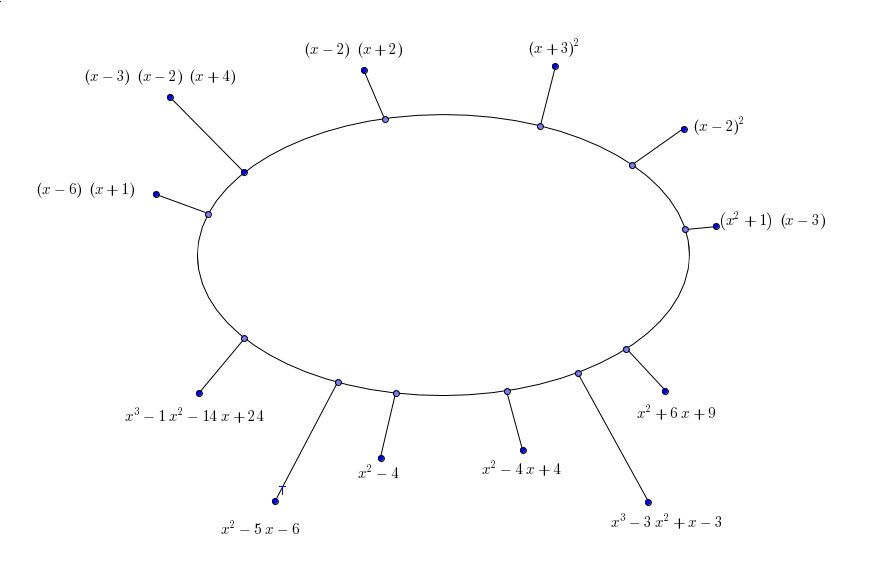
\includegraphics[scale=0.4]{img/RetoUnir.png}
\end{figure}


\subsubsection{Deberes}
\label{ses4:deberes}

\newbloq A realizar 4 de 7:

\newpreg{\hl{0}}{Calcula, sin multiplicar:
$(x-3)^2+(x+3)^2$
}

\newpreg{\hl{0}}{Calcula, sin multiplicar:
$-(x+3)^2+(x+3)(x-3) + 9$
}

\newpreg{\hl{0}}{Calcula, sin multiplicar:
$(-x+3)(-x-3)$
}

\newpreg{\hl{0}}{Calcula, sin multiplicar:
$(-x+3)^2+(-x+3)(-x-3) + 9$
}


\newpreg{\hl{0}}{Calcula, sin multiplicar:
$(x-3)^2+(x+3)^2$
}

\newpreg{\hl{0}}{Descompón la siguiente identidad notable: $x^2-2$
}

\newpreg{\hl{0}}{
	Descompón en un producto de identidades notables: $p(x) = x^4-16$
	\\\textit{Solución: $p(x) = (x^2+4)(x^2-4) = (x^2+4)(x+2)(x-2)$
	}
}



%%%%%%%%%%%%%%%%%%%%%%%%%%%%%%%%%%%%%%%%%%%%%%%%%%%%%%%%%%%%%%%%%%%
%%%%%%%%%%%%%%%%%%%%%%%%%%%%%%%%%%%%%%%%%%%%%%%%%%%%%%%%%%%%%%%%%%%
%%%%%%%%%%%%%% 			Sesión 5		%%%%%%%%%%%%%%%%%%%%%%%%%%%
%%%%%%%%%%%%%%%%%%%%%%%%%%%%%%%%%%%%%%%%%%%%%%%%%%%%%%%%%%%%%%%%%%%
%%%%%%%%%%%%%%%%%%%%%%%%%%%%%%%%%%%%%%%%%%%%%%%%%%%%%%%%%%%%%%%%%%%

\section{Sesión 5}


\paragraph{Contenidos}
\begin{itemize}
	\item Factorización. Conceptos teóricos, diferencia entre raíz y factor.
	\item Factorización utilizando: identidades notables, fórmula de resolución de ecuaciones de segundo grado, sacando factor común y aplicando los casos anteriores en polinomios de la forma: $P(x) = ax^3+bx^2+cx$.
\end{itemize}

\paragraph{Desarrollo de la sesión}

Se pone en marcha la medalla de \logro{Ojo Avizor}{avizor}.
%
Esta medalla tiene 3 subniveles y como máximo se puede ascender un nivel en cada clase.
%
Cada vez que en cualquier clase aparezca una identidad notable, cualquier alumno podrá levantar la mano para identificarla y resolverla. 
%
Si la resuelve correctamente obtendrá un subnivel del logro.

La sesión se desarrollará utilizando la exposición por parte del docente con abundantes ejemplos y ejercicios para practicar por parte de los alumnos.
%
La sesión comenzará enlazando con el final de la sesión anterior: utilización de identidades notables para encontrar los ceros un polinomio.
%
Se explicará que a estos ceros se les llama raíces y que con ellos se pueden construir factores para escribir el polinomio como un producto de términos de la forma $(x-a)$ con $a\in\real$.
%
A estos factores que se multiplican, se les llama factores y al proceso de escribir un polinomio como producto de sus factores se le denomina factorización.

A continuación se empleará todo el tiempo restante en factorizar polinomios.
%
El docente realizará primero uno utilizando un método (identidades notables) y se propondrá a los alumnos 2 polinomios para factorizar así.
%
Se realizará lo mismo con los otros 2 métodos: resolución de ecuaciones de segundo grado y factor común.

Se propone el siguiente itinerario:

\begin{itemize}
	\item Factorizar $x^4-16$. Proponer para factorizar $(x-3)·(x-2)$,$x^4-9 = (x^2+9)(x-\sqrt{3})(x+\sqrt{3})$ y $x^2+6x+9 = (x+3)^2$.
	
	\item Factorizar $x^2-5x+6$. Proponer para factorizar $x^2-2x-8 = (x-4)(x+2)$ y $2x^4-3x-2 = (2x+1)(x-2)$
	\item Factorizar $x^5-16x^3$. Proponer para factorizar $x^3-6x^2+9x = x(x-3)^2$.
	\item Si da tiempo: Factorizar $x^4+6x^2+9$. Proponer para factorizar $x^4-5x^2+6$.
\end{itemize}




%%%%%%%%%%%%%%%%%%%%%%%%%%%%%%%%%%%%%%%%%%%%%%%%%%%%%%%%%%%%%%%%%%%
%%%%%%%%%%%%%%%%%%%%%%%%%%%%%%%%%%%%%%%%%%%%%%%%%%%%%%%%%%%%%%%%%%%
%%%%%%%%%%%%%% 			Sesión 6		%%%%%%%%%%%%%%%%%%%%%%%%%%%
%%%%%%%%%%%%%%%%%%%%%%%%%%%%%%%%%%%%%%%%%%%%%%%%%%%%%%%%%%%%%%%%%%%
%%%%%%%%%%%%%%%%%%%%%%%%%%%%%%%%%%%%%%%%%%%%%%%%%%%%%%%%%%%%%%%%%%%

\section{Sesión 6}

\paragraph{Contenidos}
\begin{itemize}
	\item Algoritmo de división de Ruffini.
	\item Aplicación a la factorización.
	\subitem Atajos en la factorización.
\end{itemize}

\paragraph{Desarrollo de la sesión}

Se comenzará la sesión explicando el algoritmo de Ruffini para la división. 
%
Se comenzará diviendo $2x^3-x^4+5x-4$ entre $x-3$ (cuyo resultado es $-x^3-x^2-3x-4$ y resto $-16$).

Una vez explicado el método, se les pedirá que vuelvan a hacer el desafío de las divisiones (\ref{app:ses3:coop}) con el mismo esquema de trabajo utilizando siempre que puedan el algoritmo de Ruffini.
%
Se espera que, al realizar las mismas divisiones, se den cuenta del potencial de Ruffini como algoritmo de división.

Cuando hayan terminado se procederá a la explicación de cómo factorizar polinomios como $ p(x) = x^3+2x^2-5x-6$ cuyos factores son: $(x+1)(x-2)(x+3)$. 
%
Se explicará que es un método de prueba y error,  pero que disponemos de algunos atajos para su realización. 
%
En este polinomio, las posibles raíces enteras son los divisores del término independiente entre el coeficiente principal, es decir: $\pm1,\pm2,\pm3,\pm6$.

Una vez realizado este ejemplo, se les propondrán para que trabajen ellos los siguientes ejercicios: $x^3-x^2-x+1 = (x-1)^2(x+1)$, $x^2-4x+4 = (x-2)^2$ y $x^3-4x^2+x+6 = (x+1)(x-2)(x-3)$

Se propondrán ejercicios de deberes en \textit{edmodo} (ver \ref{ses6:deberes}) con el esquema utilizado anteriormente.
%
En estos deberes se incorporará un vídeo con la explicación teórica sobre la factorización de polinomios con coeficiente principal distinto de 1.


\subsubsection{Deberes}
\label{ses6:deberes}


\newbloq A elegir 3 de 6.

\newpreg{\hl{0}}{Factoriza, si es posible, $x^4+5x^3+5x^2-5x-6$.
\\\textit{Solución: $(x+2)(x+3)(x-1)(x+1)$
}
}

\newpreg{\hl{0}}{Factoriza, si es posible, $x^4+4x^3+6x^2-4x+1$.
\\\textit{Solución: $(x-1)^4$
}
}

\newpreg{\hl{0}}{Factoriza, si es posible, $x^2+x-42$.
\\\textit{Solución: $(x-6)(x+7)$}
}


\newpreg{\hl{0}}{Factoriza, si es posible, $x^4+x^3+x^2+x+1$.
\\\textit{No se puede factorizar.}
}

\newpreg{\hl{0}}{Factoriza, si es posible, $x^6-2x^3+1$.
\\\textit{Solución: $[(x-1)(x^2+x+1)]^2$}
}


\newpreg{\hl{0}}{Factoriza, si es posible, $x^{10}-4x^8+6x^6-4x^4+x^2$.
\\\textit{Solución: $x^2(x^2-1)^4$
}
}


%%%%%%%%%%%%%%%%%%%%%%%%%%%%%%%%%%%%%%%%%%%%%%%%%%%%%%%%%%%%%%%%%%%
%%%%%%%%%%%%%%%%%%%%%%%%%%%%%%%%%%%%%%%%%%%%%%%%%%%%%%%%%%%%%%%%%%%
%%%%%%%%%%%%%%		Sesiones 7 y 8		%%%%%%%%%%%%%%%%%%%%%%%%%%%
%%%%%%%%%%%%%%%%%%%%%%%%%%%%%%%%%%%%%%%%%%%%%%%%%%%%%%%%%%%%%%%%%%%
%%%%%%%%%%%%%%%%%%%%%%%%%%%%%%%%%%%%%%%%%%%%%%%%%%%%%%%%%%%%%%%%%%%

\section{Sesiones 7 y 8}


\paragraph{Contenidos}
\begin{itemize}
	\item Repaso de todo, incluyendo la factorización de polinomios con coeficiente principal distinto de 1.
\end{itemize}

Se les entregará el último papiro sin resolver de la investigación para que lo resuelvan.
%
Es un reto complicado que implica aplicar con soltura todos los conocimientos aprendidos además de seguir aplicando conocimiento de años anteriores.


Se dispone de 2 sesiones para su realización: la primera se trabajará individualmente (cada miembro del equipo tendrá una ficha ligeramente diferente, ver \ref{ses7:indiv}) y la segunda se trabajará cooperativamente (ver \ref{ses7:coop}).
%
Para la segunda sesión será necesario que los alumnos hayan finalizado con éxito sus partes individuales, ya que el equipo necesitará los resultados obtenidos en la parte individual.

La correcta resolución del ejercicio cooperativo les dará la parte decimal de la longitud del lugar del tesoro (en este caso $714$).
%
En caso de que no les diera tiempo a resolverlo en clase, tendrían que terminarlo por su cuenta.

De cara a la preparación del examen tendrán en \textit{edmodo} un quizz que podrán hacer a modo de auto-evaluación cuantas veces quieran.


\subsection{Reto final (sesiones 7 y 8)}
\label{ses7:indiv}

\subsubsection{Alumnos}
%!TEX root = ../TFM.tex


Todos los retos sigeun el mismo esquema, cambiando los polinomios iniciales y, por tanto, los resultados intermedios y el restultado final.
%
Cada alumno obtendrá como resultado un polinomio $A_i(x)$ necesario para el reto cooperativo.

\paragraph{Alumno 1:\\}



Tus 3 polinomios para trabajar son: $P(x) =  x^3 - 2x^2 + x - 2 $ ; $Q(x) =  x^2 - 2x - 3 $ y $R(x) =  x^2 - 5x + 6 $.



Calcula: $M(x) = P(x)\cdot  Q(x)$ (sol: $ x^5 - 4x^4 + 2x^3 + 2x^2 + x + 6 $).

Calcula: $N(x) = R(x)\cdot  Q(x)$ (sol: $ x^4 - 7x^3 + 13x^2 + 3x - 18 $).

Calcula: $D(x) = ( x + 1 )\cdot  ( x - 2 )$

Calcula: $R(x) = N(x) / D(x)$ (Solución: $ x^2 - 6x + 9 $)

Calcula: $R(x) - ( x^2 - 6x + 9 )$ (Solución: $ 0 $)

Para terminar, factoriza $M$ y $N$, sabiendo:

     [3, 2]  son raíces de $M$

     [2]  es raíz de $N$

Solución: $N(x) =  (x - 2) \cdot  (x + 1) \cdot  (x - 3)^2 $ y $M(x) =  (x - 3) \cdot  (x - 2) \cdot  (x + 1) \cdot  (x^2 + 1) $

Toma \[\frac{M}{N} = \frac{\quad\quad\quad\quad}{\quad\quad\quad\quad}\]

¿Cuáles se pueden simplificar? (Solución: $ (x - 3) \cdot  (x - 2) \cdot  (x + 1) $

Escribe todos los términos que puedas simplificar y llama $A_1(x)$ al resultado.













\paragraph{Alumno 2:\\}



Tus 3 polinomios para trabajar son: $P(x) =  x^2 - 2x - 3 $ ; $Q(x) =  x^3 - 4x $ y $R(x) =  x^2 - 5x + 6 $.



Calcula: $M(x) = P(x)\cdot  Q(x)$ (sol: $ x^5 - 2x^4 - 7x^3 + 8x^2 + 12x $).

Calcula: $N(x) = R(x)\cdot  Q(x)$ (sol: $ x^5 - 5x^4 + 2x^3 + 20x^2 - 24x $).

Calcula: $D(x) = ( x )\cdot  ( x - 3 )$

Calcula: $R(x) = N(x) / D(x)$ (Solución: $ x^3 - 2x^2 - 4x + 8 $)

Calcula: $R(x) - ( x^3 - 2x^2 - 4x + 8 )$ (Solución: $ 0 $)

Para terminar, factoriza $M$ y $N$, sabiendo:

     [3, 2]  son raíces de $M$

     [3, 0]  son raíces de $N$

Solución: $N(x) =  (x - 3) \cdot  x \cdot  (x + 2) \cdot  (x - 2)^2 $ y $M(x) =  (x - 3) \cdot  (x - 2) \cdot  x \cdot  (x + 1) \cdot  (x + 2) $

Toma \[\frac{M}{N} = \frac{\quad\quad\quad\quad}{\quad\quad\quad\quad}\]

¿Cuáles se pueden simplificar? (Solución: $ (x - 3) \cdot  (x - 2) \cdot  x \cdot  (x + 2) $

Escribe todos los términos que puedas simplificar y llama $A_2(x)$ al resultado.













\paragraph{Alumno 3:\\}



Tus 3 polinomios para trabajar son: $P(x) =  x^3 - 4x $ ; $Q(x) =  x^2 - 5x + 6 $ y $R(x) =  x^2 - 5x + 6 $.



Calcula: $M(x) = P(x)\cdot  Q(x)$ (sol: $ x^5 - 5x^4 + 2x^3 + 20x^2 - 24x $).

Calcula: $N(x) = R(x)\cdot  Q(x)$ (sol: $ x^4 - 10x^3 + 37x^2 - 60x + 36 $).

Calcula: $D(x) = ( x - 2 )\cdot  ( x - 3 )$

Calcula: $R(x) = N(x) / D(x)$ (Solución: $ x^2 - 5x + 6 $)

Calcula: $R(x) - ( x^2 - 5x + 6 )$ (Solución: $ 0 $)

Para terminar, factoriza $M$ y $N$, sabiendo:

     [3, 0]  son raíces de $M$

     [3]  es raíz de $N$

Solución: $N(x) =  (x - 3)^2 \cdot  (x - 2)^2 $ y $M(x) =  (x - 3) \cdot  x \cdot  (x + 2) \cdot  (x - 2)^2 $

Toma \[\frac{M}{N} = \frac{\quad\quad\quad\quad}{\quad\quad\quad\quad}\]

¿Cuáles se pueden simplificar? (Solución: $ (x - 3) \cdot  (x - 2)^2 $

Escribe todos los términos que puedas simplificar y llama $A_3(x)$ al resultado.













\paragraph{Alumno 4:\\}



Tus 3 polinomios para trabajar son: $P(x) =  x^2 - 5x + 6 $ ; $Q(x) =  x^3 - 2x^2 + x - 2 $ y $R(x) =  x^2 - 5x + 6 $.



Calcula: $M(x) = P(x)\cdot  Q(x)$ (sol: $ x^5 - 7x^4 + 17x^3 - 19x^2 + 16x - 12 $).

Calcula: $N(x) = R(x)\cdot  Q(x)$ (sol: $ x^5 - 7x^4 + 17x^3 - 19x^2 + 16x - 12 $).

Calcula: $D(x) = ( x - 2 )\cdot  ( x - 3 )$

Calcula: $R(x) = N(x) / D(x)$ (Solución: $ x^3 - 2x^2 + x - 2 $)

Calcula: $R(x) - ( x^3 - 2x^2 + x - 2 )$ (Solución: $ 0 $)

Para terminar, factoriza $M$ y $N$, sabiendo:

     [3, 2]  son raíces de $M$

     [3, 2]  son raíces de $N$

Solución: $N(x) =  (x - 3) \cdot  (x - 2)^2 \cdot  (x^2 + 1) $ y $M(x) =  (x - 3) \cdot  (x - 2)^2 \cdot  (x^2 + 1) $

Toma \[\frac{M}{N} = \frac{\quad\quad\quad\quad}{\quad\quad\quad\quad}\]

¿Cuáles se pueden simplificar? (Solución: $ (x - 3) \cdot  (x - 2)^2 \cdot  (x^2 + 1) $

Escribe todos los términos que puedas simplificar y llama $A_4(x)$ al resultado.








\subsubsection{Parte cooperativa}
\label{ses7:coop}

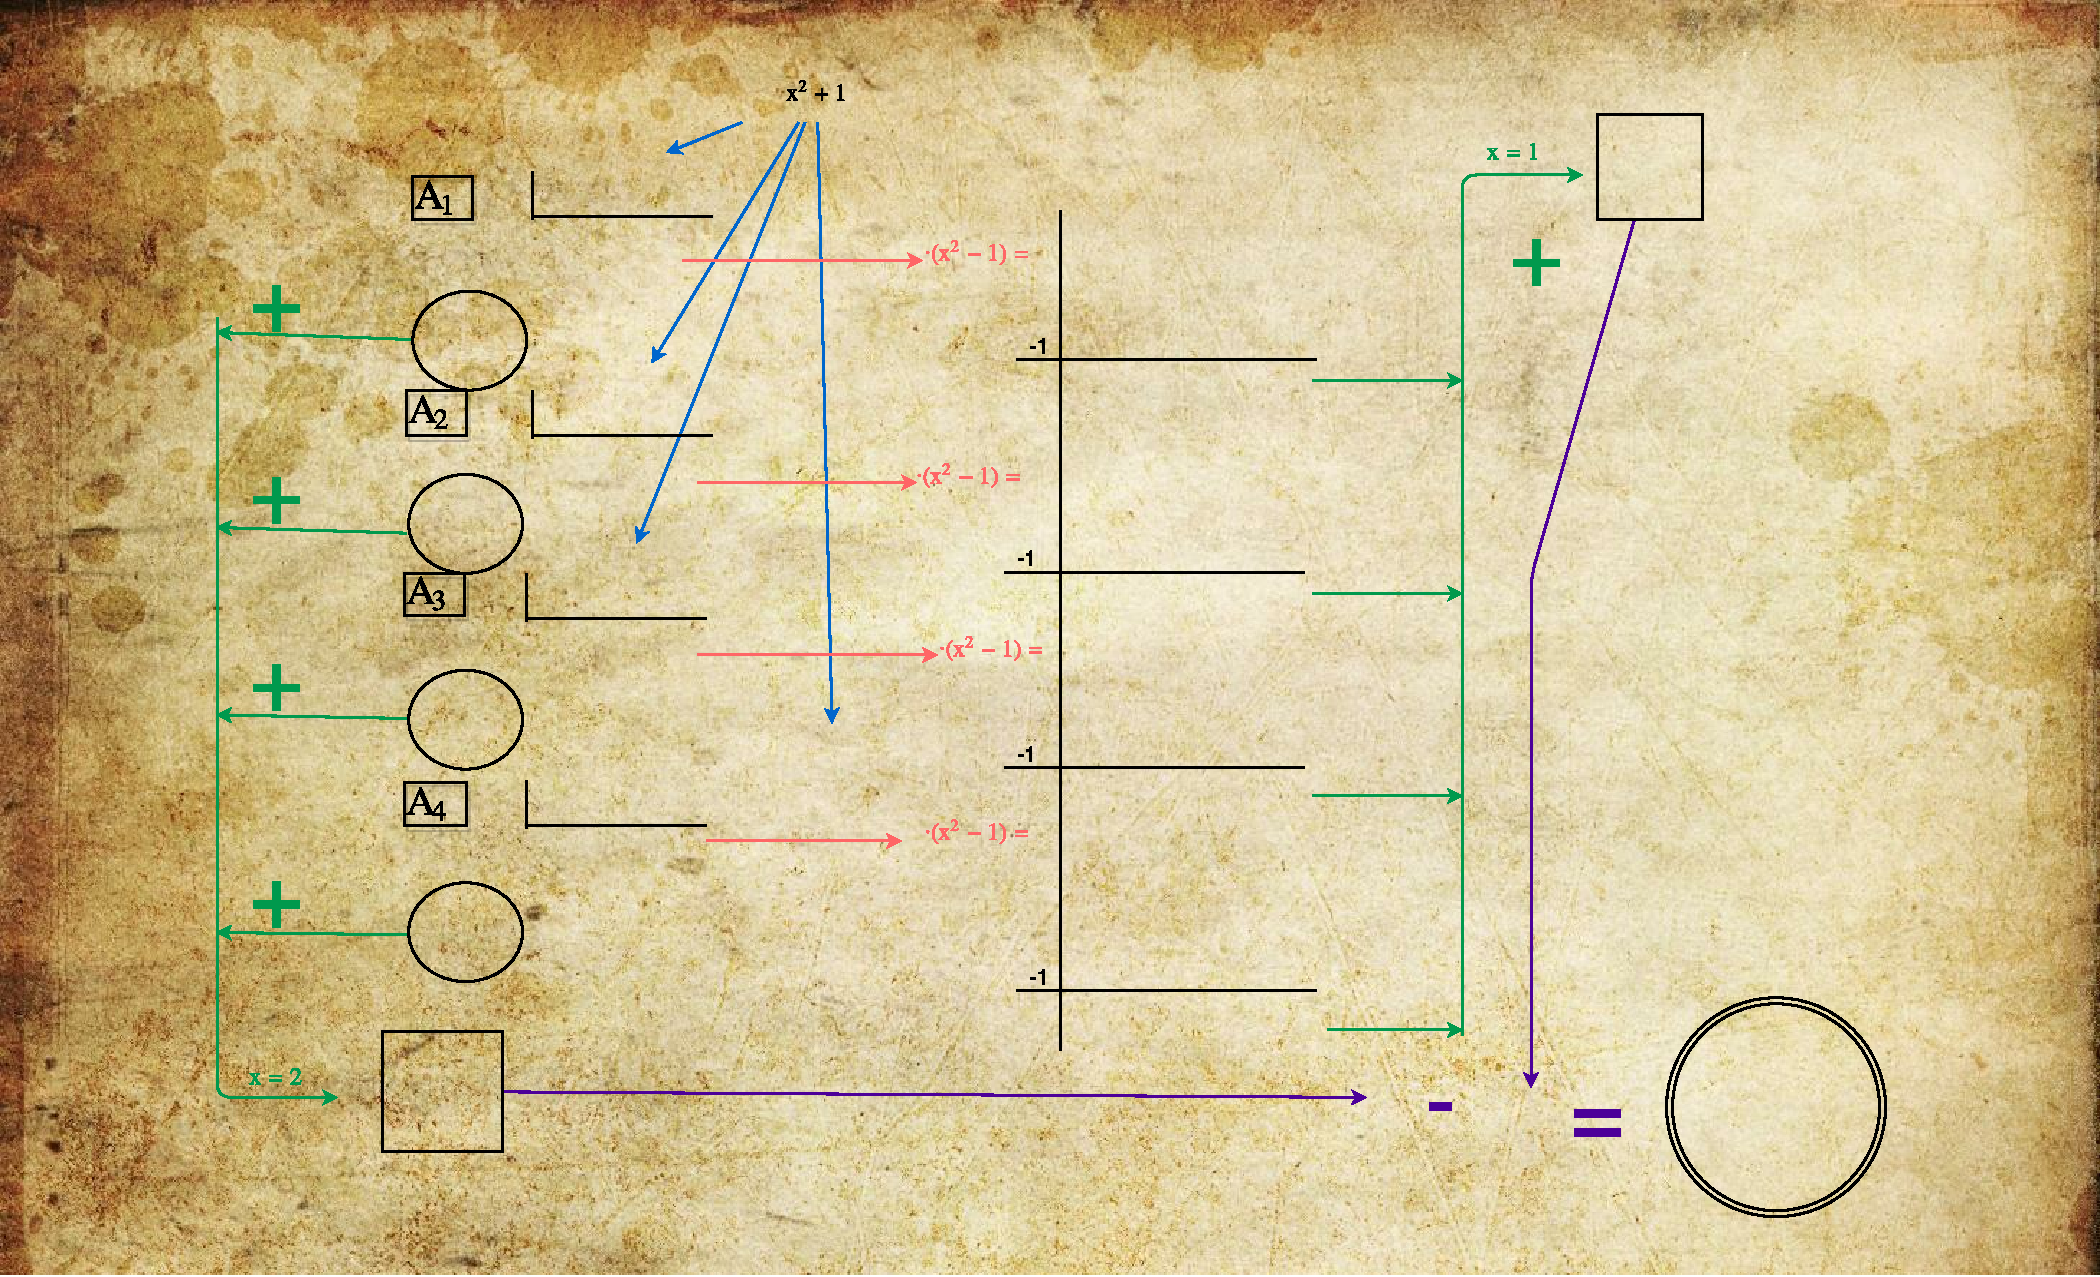
\includepdf[pages={1},pagecommand={},width=1.05\textheight,landscape=true]{src/RetoCoop.pdf}




%%%%%%%%%%%%%%%%%%%%%%%%%%%%%%%%%%%%%%%%%%%%%%%%%%%%%%%%%%%%%%%%%%%
%%%%%%%%%%%%%%%%%%%%%%%%%%%%%%%%%%%%%%%%%%%%%%%%%%%%%%%%%%%%%%%%%%%
%%%%%%%%%%%%%% 			Sesión 9		%%%%%%%%%%%%%%%%%%%%%%%%%%%
%%%%%%%%%%%%%%%%%%%%%%%%%%%%%%%%%%%%%%%%%%%%%%%%%%%%%%%%%%%%%%%%%%%
%%%%%%%%%%%%%%%%%%%%%%%%%%%%%%%%%%%%%%%%%%%%%%%%%%%%%%%%%%%%%%%%%%%

\section{Sesión 9}


En esta sesión, no necesariamente la sesión siguiente a la sesión 8, tendrá lugar el examen de la unidad (si se considera que haya un examen para esta unidad\crossref{, ver \ref{eval}}).
%
Los ejercicios propuestos para el examen se encuentran en \ref{examen}.


\subsection{Examen}
\label{examen}

\includepdf[pages=-,pagecommand={},width=1.22\textwidth]{pdf/Examen.pdf}


\subsection{Autoevaluación}
\label{app:autoeval}

Se propone para la autoevaluación del libro de apoyo \cite[p. 120]{MareaVerde} además de la realización de los ejercicios propuestos de deberes que no se hayan realizado a lo largo de la Unidad Didáctica.

\includepdf[pages={120},pagecommand={},width=1.2\textwidth]{pdf/3ESOBCompletoLOMCE.pdf}




\cleardoublepage
\ifinapp

  \chapter{Documentos adjuntos}

  A continuación, se presenta el apéndice de los documentos completos mencionados a lo largo del trabajo.
  %
  Esto es, los retos de las sesiones 1,2,3 (Introducción, multiplicación y división de polinomios respectivamente).
  %
  Seguido, se encuentra el reto cooperativo final.
  %
  Por último, encontramos los documentos correspondientes al examen y la autoevaluación propuestos para esta Unidad Didáctica.


  \cleardoublepage
  \rhead{}
  \lhead{}
  \chead{Reto de la primera sesión (Introducción)}
  \label{app:retoses2}
  \includepdf[pages=-,pagecommand={},width=1.4\textwidth]{src/RetoSes1.pdf}

  \cleardoublepage
  \chead{Reto de la sesión 2 (Multiplicación de polinomios)}
  \label{app:retomulti}
  \includepdf[pages=-,pagecommand={},width=1.05\textheight,landscape=true]{src/RetoMulti.pdf}

  \cleardoublepage
  \chead{Reto de la sesión 3 (División de polinomios)}
  \label{app:retodivi}
  \includepdf[pages=-,pagecommand={},width=1.05\textheight,landscape=true]{src/RetoDivision.pdf}


  \cleardoublepage
  \chead{Reto de las sesiones 7 y 8 (Repaso general)}
  \label{app:retocoop}
  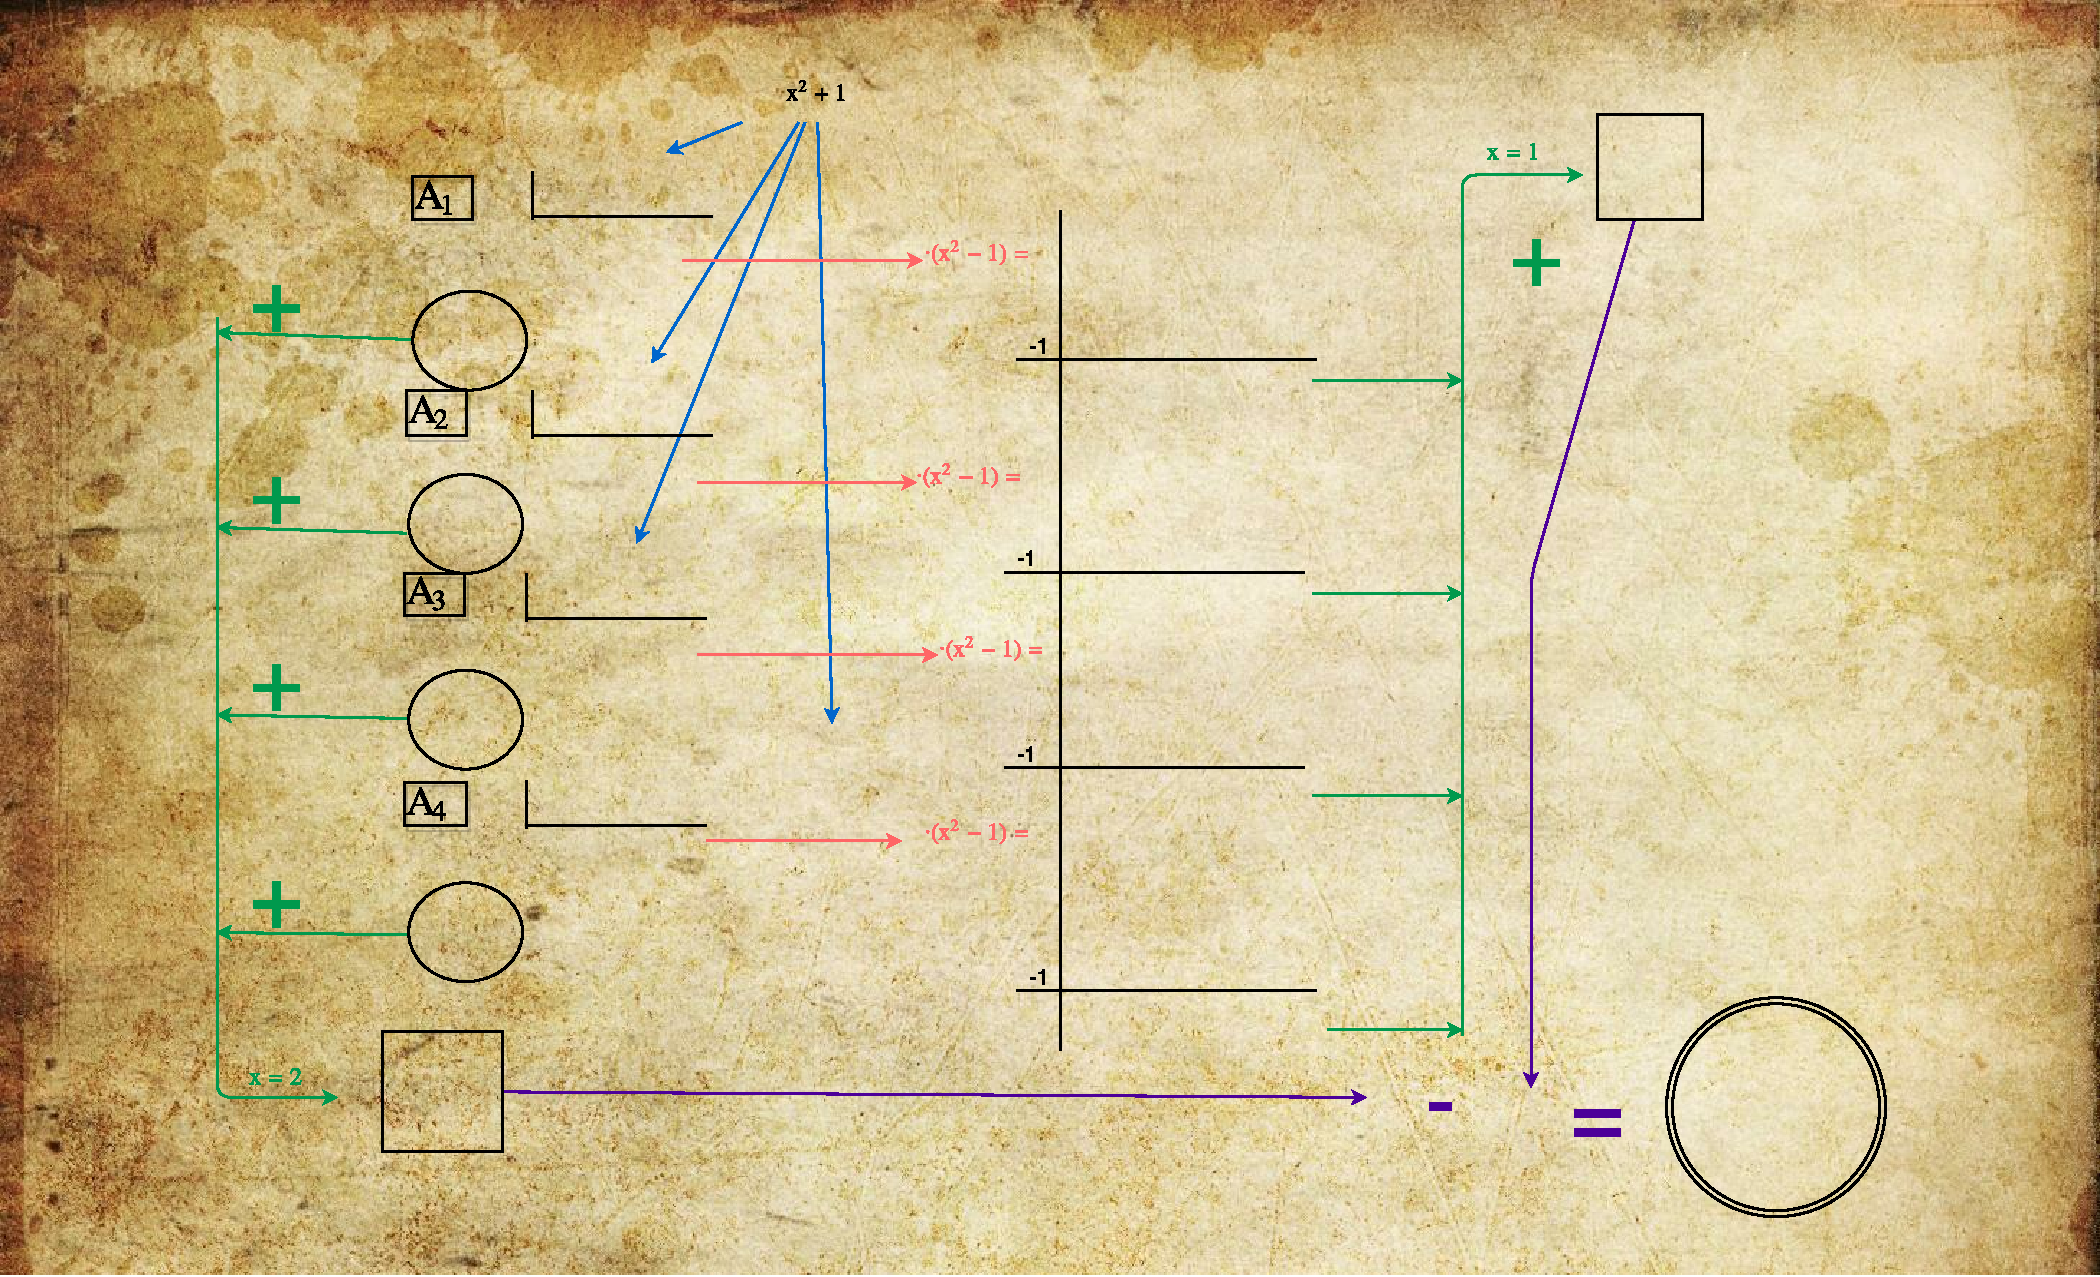
\includepdf[pages={1},pagecommand={},width=1.05\textheight,landscape=true]{src/RetoCoop.pdf}

  \cleardoublepage
  \chead{Examen propuesto para la Unidad Didáctica}
  \label{app:examen}
  \includepdf[pages=-,pagecommand={},width=1.22\textwidth]{pdf/Examen.pdf}

  \cleardoublepage
  \chead{Autoevaluación propuesta para la Unidad Didáctica}
  \label{app:autoeval}
  \includepdf[pages={120},pagecommand={},width=1.2\textwidth]{pdf/3ESOBCompletoLOMCE.pdf}

  \chead{\centerhead}
  \rhead{\righthead}
  \lhead{\lefthead}

\fi

\chapter{Recursos adicionales}




\chapter{Recursos adicionales}

\section{Generador de los retos}

Los retos se han diseñado utilizando la herramienta \url{draw.io}.

\defcitealias{Sage}{cocalc.com}

El código se puede probar online en \citetalias{Sage} \footnote{Simulador de Sage Online.}


\begin{python}
# Definicion del cuerpo de trabajo: Los racionales.
R.<x> = QQ[]

P1 = (x^2+1)*(x-2)
P2 = (x+1)*(x-3)
P3 = (x - 2) * x * (x + 2)
P4 = (x-2)*(x-3)

LP = [P1,P2,P3,P4]
numRetos=4

#### Definiciones auxiliares.
def _expand(P):
    _A = x^2+x+1
    if (type(P) == type(_A.factor())):
        return P.expand()
    else:
        return P

def _simplificable(P,Q):
    return P.gcd(Q).factor()

def _RootsTil(P,n):
    ret = []
    [ret.append(P.roots()[i][0]) for i in range(0,P.degree()-n)]
    return ret

def reto_indiv(_P,_Q,Contador):
    print "ESTE ES EL RETO ",Contador
    
    P = _expand(_P)
    Q = _expand(_Q)
    R = _expand(P.factor()[0][0]*Q.factor()[0][0])
    
    print "Tus 3 polinomios para trabajar son: P(x) = ",P," ; Q(x) = ",Q," y R(x) = ",R,".\n"
    
    M = P*Q
    print "Calcula: M(x) = P(x)Q(x) (sol: ",M,")."

    N = R*Q
    print "Calcula: N(x) = R(x)Q(x) (sol: ",N,")."

    D = N.factor()[1][0]*N.factor()[0][0]
    print "Calcula: D(x) = (",N.factor()[1][0],")(",N.factor()[0][0],")"

    R=N/D
    print "Calcula: R(x) = N(x) / D(x) (Sol: ",R,")\n Calcula: R(x) - (",R,") (Sol: ",R-R,")"

    
    print "Para terminar, factoriza M y N, sabiendo:"
    a = _RootsTil(M,3)
    if len(a) == 1:
        print "    ",a," es raiz de M"
    else:
        print "    ",a," son raices de M"
    
    a=_RootsTil(N,3)
    if len(a) == 1:
        print "    ",a," es raiz de N"
    else:
        print "    ",a," son raices de N"
    
    print "Sol: N(x) = ",N.factor()," y M(x) = ",M.factor(),""
        
    retval = _simplificable(M,N)
    print "Indica si hay algo que se pueda simplificar en M(x)/N(x) (Sol: ",retval,")"
    
    print "Escribe todos los terminos que puedas simplificar y llama $A_%d$ al resultado.\n\n\n\n\n"%Contador   
    return retval


#### Main

A = []
for i in xrange(numRetos): 
    A.append(reto_indiv(LP[i],LP[(i+1)%numRetos],i+1))
    

c=0
CS=[]
for i in xrange(len(A)):
    print "Poli: ",_expand(A[i])
    print "Divide por $D(x) = x^2+1$"
    print "Cociente: ",CS.append(_expand(A[i])//(x^2+1))
    f=_expand(A[i])//(x^2+1)
    print "Resto: ",_expand(A[i])%(x^2+1)
    c=c+f(6.177)
    print ""

print "Multiplica (x^2-1) y divide por x+1 y evalua en 1"
[(CS[i]*(x^2-1)/(x+1))(1) for i in range(len(CS))]

\end{python}



%%%%%%%%%%%%%%%%%%%%%%%%%%%%%%%%%%%%%%%%%%%%%%%%%%%%%%%%%%%%%%%%%%%%%%%%%%%%%%%%
%%%%%%%%%%%%%%%%%%%%%%%%%%%%%%%%%%%%%%%%%%%%%%%%%%%%%%%%%%%%%%%%%%%%%%%%%%%%%%%%
% BIBLIOGRAFIA %
%%%%%%%%%%%%%%%%%%%%%%%%%%%%%%%%%%%%%%%%%%%%%%%%%%%%%%%%%%%%%%%%%%%%%%%%%%%%%%%%

\cleardoublepage

% Las siguientes dos instrucciones es todo lo que necesitas
% para incluir las citas en la memoria
\bibliography{memoria}  % memoria.bib es el nombre del fichero que contiene
% las referencias bibliográficas. Abre ese fichero y mira el formato que tiene,
% que se conoce como BibTeX. Hay muchos sitios que exportan referencias en
% formato BibTeX. Prueba a buscar en http://scholar.google.com por referencias
% y verás que lo puedes hacer de manera sencilla.
% Más información: 
% http://texblog.org/2014/04/22/using-google-scholar-to-download-bibtex-citations/

\ifincgls
\printindex
\fi

\end{document}
